\documentclass[conference]{IEEEtran}
%\IEEEoverridecommandlockouts
% The preceding line is only needed to identify funding in the first footnote. If that is unneeded, please comment it out.
%% \usepackage{cite}
\usepackage{hyperref}
\usepackage{svg}

\usepackage{amsmath,amssymb,amsfonts}
\usepackage{amsthm} % Allows usage of '\theoremstyle'

\usepackage{algorithmic}
\usepackage{graphicx}
\usepackage{textcomp}
\usepackage{xcolor}
\usepackage{subcaption}
\usepackage[font=small,labelfont=bf]{caption} % small fontsize in caption

\usepackage{siunitx}

%% \def\BibTeX{{\rm B\kern-.05em{\sc i\kern-.025em b}\kern-.08em
%%     T\kern-.1667em\lower.7ex\hbox{E}\kern-.125emX}}

\usepackage[
    backend=biber,
    style=ieee,
    sorting=none,
    %% citestyle=authoryear
    ]{biblatex}
\addbibresource{bibliography.bib}

\usepackage[normalem]{ulem}


\begin{document}
\newcommand{\vect}[1]{\boldsymbol{#1}}
\newcommand{\vecs}[1]{\boldsymbol{#1}}
\newcommand{\matr}[1]{\boldsymbol{#1}}
\newcommand{\matd}[1]{\mathcal{#1}}
% \newcommand{\matd}[1]{\boldsymbol{#1}^{d}}

\newcommand{\dotprod}[2]{\left\langle {#1}, \, {#2} \right\rangle}
\newcommand{\normdotprod}[2]{\frac{\left\langle #1, \, #2 \right\rangle}{\| #1 \| \, \| #2 \|}}


\newtheorem{theorem}{Theorem}[section]
\newtheorem{corollary}{Corollary}[section]
\newtheorem{lemma}{Lemma}[section]
% \theoremstyle{definition}
\newtheorem{definition}{Definition}[section]

\newif\ifthesis
\thesisfalse

\title{
Passive Obstacle Aware Control \\
to Follow Desired Velocities
}

\author{
  \IEEEauthorblockN{Lukas Huber$^{1}$, Trinca Thibaud$^{1}$, Jean-Jacques Slotine$^{2}$, Aude Billard$^{1}$}
\thanks{This work was supported by EU ERC grant SAHR.} %Use only for final RAL version
\thanks{$^{1}$LASA Laboratory, Swiss Federal School of Technology in Lausanne - EPFL, Switzerland. \tt $\{$lukas.huber;aude.billard$\}$@epfl.ch }
\thanks{$^{2}$Nonlinear Systems Laboratory,  Massachusetts Institute of Technology, USA. \tt jjs@mit.edu}   %\tt \small
% \thanks{Manuscript received: May 10, 2022; Revised November 7, 2022; December 14, 2022.}%Use only for final RAL version
% \thanks{This paper was recommended for publication by Editor Aniket Bera.}
% \thanks{Digital Object Identifier (DOI): see top of this page.}
}


\maketitle
\thispagestyle{plain}
\pagestyle{plain}
    
\begin{abstract}
Evaluating and updating the obstacle avoidance velocity for an autonomous robot in real-time ensures robustness against noise and disturbances. A passive damping controller can obtain the desired motion with a torque-controlled robot, which remains compliant and ensures a safe response to external perturbations.
Here, we propose a novel approach for designing the passive control policy. 
Our algorithm complies with obstacle-free zones while transitioning to increased damping near obstacles to ensure collision avoidance. 
This approach ensures stability across diverse scenarios, effectively mitigating disturbances.
Validation on a 7DoF robot arm demonstrates superior collision rejection capabilities compared to the baseline, underlining its practicality for real-world applications. 
Our obstacle-aware damping controller represents a substantial advancement in secure robot control within complex and uncertain environments.
\end{abstract}

\begin{IEEEkeywords}
Obstacle avoidance, dynamical systems, passivity, compliant control, human-robot interaction
\end{IEEEkeywords}

% Test
% \begin{equation}
% 	\mathcal{S}(\vecs \xi) = \text{diag} \left(s_1 , \; .., \; s_N \right) 
% \end{equation}

\section{Introduction}
Robots moving in real-world scenarios need to be adaptable and reactive.
While on the one hand, the robot needs to complete its motion, on the other hand, its movement must be safe, i.e., it can avoid collisions at all times.
Modern robotic applications require increased physical human-robot collaboration \cite{ajoudani2018progress}.

One of the big tasks of controlling a robot is planning a trajectory to reach a desired goal. Trajectories can often be very complex, and one has to find methods to parametrize those easily. The human demonstration is an easy way of showing the robot what to do. Simple movement can be sequenced to generate a complex motion \cite{gribovskaya2011motion}.

It has a closed-form control law does not require constant replanning for every position. In addition, DS control can provide stability and convergence guarantees for navigation in dynamic environments.

Applications that involve interactions with an unknown and dynamic environment, for example, manipulation around humans, require controllers for actuators that are not which exceed classical stiffness controllers.

Biological muscles outperform mechanical devices in terms of functional and neuro-mechanical control. One key distinction is the adaptable compliance or variable stiffness exhibited in biological systems, which contrasts with the performance of traditional stiff electrical drives commonly used in industrial robotics. Unlike these drives, which rely on precise reference-trajectory tracking, biological systems possess inherent flexibility and adaptability.

Most reactive motion controllers do not specifically consider the task of obstacle avoidance. This is the advantage of impedance controllers; if designed correctly, the motion remains stable for collision avoidance. Additionally, the force applied to an external obstacle remains below a specified threshold. 
However, for improved behavior, the robot should avoid collisions proactively before they happen while the impedance control remains in the fail-safe interaction mode.

\begin{figure}
\centerline{\includegraphics[width=0.5\textwidth]{figures/robot_arm_table_avoidance}}
\caption{Using the proposed obstacle aware passivity controller, the robot is able to safely avoid external disturbance and ensuring collision avoidance.}
\label{fig:table_avoidance_with_obstacle}
\end{figure}


\subsection{Literature Review}
\cite{takegaki1981new}
Impedance control is a feedback control algorithm that imposes a Cartesian impedance to the end-point of a nonlinear manipulator resulting \cite{hogan1985impedance}. This results in the elimination of the \textit{inverse kinematics problem} in favor of \textit{forward kinematics}.
Conversely, to position control algorithms, impedance control creates a dynamic relation between desired position, velocity, and force rather than controlling for these values individually.   
While the first impedance controller used constant stiffness, many approaches have been proposed for dynamic control parameters to have improved adaptation to the environment \cite{vanderborght2013variable, abu2020variable}. 
% older variable actuators focused review \cite{vanderborght2013variable}
% Progress and prospects of the human-robot collaboration \cite{ajoudani2018progress}

% Passive Controllers
Passive velocity field controllers first encode the desired task as a velocity field, approximating a damping control law, which tries to approximate the velocity \cite{li1999passive,}. However, the approach relies on a storage tank inspired by a virtual flywheel.

The approach is extended by providing more intuitive energy tanks to enable interaction with obstacles below the force limit \cite{kishi2003passive}.

The most recent approach uses impedance control based on selective dissipation of the energy \cite{kronander2015passive}. This method, called passive interaction control, allows the robot to be stiff or compliant depending on the direction of the disturbance.

Passivity analysis is often used for teleoperated systems to ensure safe operation during operation.
The first approach to the dynamics is slowly updating the desired position, coupled with a spring-damper model with an impedance controller for an interactive system
\cite{lee2010passive}.
A sampling-based approach has been used to provide passivity to a coupled system by analyzing the preserving passivity for the systems individually \cite{stramigioli2005sampled}.

Learning and continuously adapting the control parameters have been shown to improve the controller performance in direct human-robot collaboration
\cite{gribovskaya2011motion}.
However, the controller adaptation focuses on improving movement accuracy rather than rejecting disturbances.

A general framework can be used to ensure that position-, torque-, and impedance controllers exhibit passive \cite{albu2007unified}. By interpreting the torque feedback as the shaping of the motor inertia, the flexible robot arms can be used in complex interaction tasks, such as insertion or wiping.
Combining impedance controllers with admittance controllers allows for accurate yet cooperative control
\cite{fujiki2022series}.


% Energy tanks 
Impedance controllers are designed with time-varying stiffness to adapt the behavior from free motion to physical interaction with the environment  \cite{ferraguti2013tank}. However, such a system can become unstable, but virtual energy tanks can be used to ensure passivity.
Alternative approaches ensure the stability of variable impedance controllers by setting constraints on the damping and stiffness, as well as their rate of change \cite{kronander2016stability}.
% The controller was extended to have variable stiffness to favor task completion \cite{kronander2015passive}. However, both approaches rely on energy tanks for general, desired dynamics and do not give any guarantees in the presence of obstacles.


% Geometric Methods
Tracking controllers often require linearization or other simplification methods. However, \cite{udwadia2003new} develops a class of tracking controllers for exact control of the nonlinear mechanical systems at a low computational cost by reformulating control problems as a particular class of optimal controllers. With this method, several standard control problems in robotics can be derived \cite{peters2008unifying}.

The consistent combination of local Riemannian Motion Policies (RMP) is combined for globally stable force-controlled motion \cite{cheng2020rmp}.
New position-dependent Riemannian metrics improve the task design using RMP, allowing for reactive force control under constraints \cite{bylard2021composable}.

Geometric fabrics have been introduced as a mathematical tool for shaping the robot's nominal behavior, capturing constraints such as obstacle avoidance, joint limits, redundancy resolution
\cite{xie2020geometric}.
Finsler geometry combined with geometric fabrics has enabled increased path consistency \cite{ratliff2021generalized}.
Geometric fabric generalizes classical mechanical systems to form new physical behavior, which has been used for multi-obstacle avoidance on a 7DoF robot arm \cite{van2022geometric}.
However, the geometric methods remain challenging to parameterize and can create unwanted motion artifacts.
 
% Real-time perception meets reactive motion generation \cite{kappler2018real} -> no real feedback on the collision avoidance level ?!

% AFP / Obstacle avoidance / Motion Control
In dynamic environments, obstacle avoidance is crucial for safe navigation. Early approaches used repulsive force fields from robots to avoid collisions of robotic manipulators \cite{khatib1987unified}. 
As this approach is prone to local minima, the elastic band's method has been introduced. Interpreting the initial trajectory as an elastic band and stretching the path around obstacles improves convergence  
\cite{
brock2002task, % Corresponding conference paper
brock2002elastic}.
Passive controllers have been designed to track the curve of the general potential field. The controller compensates for Coriolis and centrifugal forces. However, the method does not provide insurance of disturbance repulsion around obstacles \cite{duindam2004passive}. 
The additional usage of circular fields \cite{singh1996real} allows force-controlled navigation in cluttered environments with increased convergence for simple obstacles
\cite{haddadin2011dynamic}.
This has been combined with force-controlled navigation for manipulators \cite{tulbure2020closing}. However, the method was limited to convex meshes and cannot guarantee the absence of local minima in space.

% Dynamical system based avoidance + control
Alternatively, in our previous work \cite{huber2019avoidance, huber2023avoidance}, we introduced collision avoidance inspired by a harmonic potential. We ensured the absence of local minima in free space and enabled navigation around complex scenarios with star-shaped obstacles.
For implementation on the real robot, a passive controller stays close to the initial dynamics \cite{kronander2015passive}. However, the passive controller does not take into account its physical surrounding, and disturbances in the proximity of obstacles could lead to collisions.

Although DS passive-controlled robots work well in some simple cases, they do not yet have a reliable way of safely navigating through an obstacle environment. This issue could lead to collisions if unknown disturbances push the agent toward an obstacle. This work presents a method to address this problem by modifying the passive control law design. The resulting controller is now aware of its environment.

\subsection{Contribution}
In this work, we introduce the following contributions:
\begin{itemize}
\item A passive controller which ensures obstacle avoidance (Section~\ref{sec:obstacle_aware_passivity})
\item A passivity analysis without the need for storage tank which holds for a general damping controller for stable vector fields (Theorem~\ref{theorem:passivity})
\item A collision avoidance analysis which provides insight into the path consistency around obstacles (Section~\ref{sec:collision_avoidance})
\item Implementation and test on real robots (Section~\ref{sec:evaluation})
\end{itemize}

\subsection{Related Work}

\subsubsection{Force Control}
Impedance control, a powerful feedback algorithm, effectively applies Cartesian impedance to nonlinear manipulators' end-points \parencite{takegaki1981new, hogan1985impedance}. The controller replaces the computationally intensive \textit{inverse kinematics} with the more straightforward \textit{forward kinematics}. Impedance control establishes a dynamic relationship between desired position, velocity, and force, offering a holistic control framework.
Initially, impedance controllers employed constant stiffness, but researchers have explored various dynamic control parameter approaches to enhance adaptability in complex environments \parencite{vanderborght2013variable, abu2020variable}. However, introducing dynamic parameters into the control framework requires taking special care of the system's stability.
Furthermore, admittance control is designed to adapt to external forces, while remaining stable contact \parencite{glosser1994implementation}. Admittance control can be interpreted as a special type of impedance control.

% Passivity with increased precision
Passive velocity controllers use a state-dependent velocity, which is converted into a control force through a damping control law. Since the controllers have variable damping parameters, stability can be guaranteed using storage tanks inspired by a virtual flywheel \parencite{li1999passive}. 
Furthermore, complex control parameters can be learned from human demonstrations. By continuously adapting the parameters, the controller can be observed to improve its tracking performance in direct human-robot collaboration tasks \parencite{gribovskaya2011motion}.
However, high compliance often results in decreased motion following. Yet, carefully designing the damping matrix, which increases stiffness in the direction of motion, but remains compliant otherwise, results in improved convergence \parencite{kronander2015passive}. 
Combining impedance controllers with admittance controllers can be used to increase accuracy in cooperative control
\parencite{fujiki2022series}.
However, these controllers' adaptations focus on improving movement accuracy rather than actively rejecting disturbances.

\iflong
% Stable interaction controller
Impedance controllers play an important role in interaction tasks, as in these situations, the robot is subjected to forces that are hard to predict precisely. However, they must be actively managed to ensure stable contact without damage occurring. In these situations, passive controllers using storage tanks based on the system's energy allow to limit contact force \parencite{kishi2003passive}.
A general framework can be used to ensure that position-, torque-, and impedance controllers exhibit passivity during interaction tasks. This is achieved by interpreting the torque feedback as the shaping of the motor inertia. It allows the use of flexible robot arms for complex interaction tasks, such as insertion or wiping \parencite{albu2007unified}. 
By sensing the interaction force and actively adapting the trajectory based on the physical interaction force and the virtual repulsive force from the obstacle. This can be used for obstacle-aware motion generation \parencite{haddadin2010real}.
\fi

\iflong
% Telemanipulation
Teleoperated systems of robot arms come with control delays and require a closed-loop controller of the robot that can adapt autonomously, ensuring stable and reliable performance. Passive controllers present themselves perfectly for such a task  \parencite{stramigioli2005sampled}. This method addresses the intricate dynamics of interactive systems, ensuring stable and reliable performance.
A similar approach involves slowly updating the desired position while incorporating a spring-damper model through an impedance controller, enabling seamless interaction with the teleoperated robotic system \parencite{lee2010passive}.
However, these models require human input for active collision avoidance.
\fi

% Energy tanks 
Many impedance controllers with time-varying control rely on energy tanks to ensure stability. This is a virtual state of the system, which is filled or emptied depending on the controller command. Limiting the energy tank to a maximum value ensures the system's stability  \parencite{ferraguti2013tank}. However, when this limit is reached, the controller is constrained and interferes with the controller's optimal functioning. This can result in the controller not achieving a main functionality, such as collision avoidance.
Alternatively, the impedance controller variables can be constrained by adapting the damping and stiffness, as well as their rate of change based on a Lyapunov function \cite{kronander2016stability}.

\subsubsection{Obstacle Avoidance}
% AFP / Obstacle avoidance / Motion Control
In dynamic environments, obstacle avoidance has to be quickly evaluated to ensure safe robot navigation. Repulsive force fields pointing away from obstacles can be used to create a collision-free motion \parencite{khatib1987unified}. 
However, these artificial potential fields are susceptible to local minima, which led to the introduction of navigation functions. A global function that combines the repulsive force fields while ensuring a global minimum and the goal \parencite{koditschek1990robot}. However, such functions depend on the distribution of the obstacles and are hard to adapt to dynamic environments and high dimensional spaces \parencite{loizou2022mobile}.


% \cite{brock2002task}, % Corresponding conference 
Passive controllers can also be used to track the desired motion of the artificial potential field while compensating for Coriolis and centrifugal forces \parencite{duindam2004passive}. 
Nonetheless, these methods lack the guarantee of disturbance repulsion around obstacles, which is addressed by the integration of circular fields, which rotates the robot's path around the obstacles \parencite{singh1996real}. 
This allows force-controlled navigation in cluttered environments, yielding convergence for simple obstacles \parencite{haddadin2011dynamic}. 
Conversely, repulsive fields can be combined with elastic, global planning \parencite{brock2002elastic} for improved convergence. This allowed adding a repulsive force from the obstacle, ensuring collision avoidance \parencite{tulbure2020closing}. 
However, methods based on artificial potential fields are prone to local minima in space around cluttered environments.

\iflong
% Geometric Methods for Obstacle Avoidance / Force Control
Traditional tracking controllers often require complex linearization or simplification methods. However, a class of geometric tracking controllers enables exact control of nonlinear mechanical systems with low computational cost \parencite{udwadia2003new}. By reformulating control problems as a specific class of optimal controllers, this approach facilitates the derivation of standard control problems in robotics \parencite{peters2008unifying}. As a result, many geometric controllers directly output a control force, and hence do not rely on an additional (impedance) controller.
Integrating local Riemannian Motion Policies (RMP) has led to globally stable force-controlled motion \parencite{cheng2020rmp}. Moreover, advancements in position-dependent Riemannian metrics allow for improved task design using RMP and reactive force control under constraints \parencite{bylard2021composable}.
Geometric fabrics have emerged as a valuable mathematical tool for shaping a robot's nominal behavior while capturing essential constraints like obstacle avoidance, joint limits, and redundancy resolution \parencite{xie2020geometric}. Combining Finsler geometry and geometric fabrics has further enhanced path consistency \parencite{ratliff2021generalized}.
Integrating geometric fabric methods into classical mechanical systems has enabled various physical behaviors, notably exemplified in multi-obstacle avoidance for a 7DoF robot arm \parencite{van2022geometric}. Despite these significant achievements, the parametrization of geometric methods and their application to general systems remains challenging and hinders their wide acceptance.
\fi

% Dynamical system based avoidance + control
Harmonic potential functions can ensure the absence of local minima in free space \parencite{connolly1997harmonic}. In previous work, we combined harmonic potential functions with the dynamical system framework to obtain reactive, local minima-free motion \parencite{huber2019avoidance, huber2023avoidance}. It allows for generating a desired velocity based on the robot's position in real-time.
For implementation on a torque-controlled robot arm, we utilized a passive controller that closely adheres to the desired velocity \parencite{kronander2015passive}. However, one of the limitations of the passive controller is its inability to  account for the physical surroundings. This makes the robot susceptible to disturbances close to obstacles, potentially leading to collisions.

Although DS passive-controlled robots work well in interactive scenarios, they cannot ensure they navigate through an obstacle environment collision-free. For example, they often give in when being pushed toward an obstacle. This work presents a method to address this problem by modifying the passive control law design, making the controller aware of its environment.
\subsection{Contribution}
We introduce a passive controller that incorporates into the feedback control loop as visualized in Figure~\ref{fig:control_scheme_passive}. 
In this work, we make the following contributions:
\begin{itemize}
\item The design of the obstacle-aware passive controller
(Section~\ref{sec:obstacle_aware_passivity})
\item A passivity guarantee (without the need for a storage tank) which applies to general damping controllers (Theorem~\ref{theorem:passivity})
\ifthesis
{}
\else
\item A collision avoidance analysis which provides insight into the path consistency around obstacles (Section~\ref{sec:collision_avoidance})
\fi
\item Discrete-time analysis to enable control parameter design which ensures stability (Section~\ref{sec:discrete_time_behavior})
\item Implementation and testing on 7DoF robot arm (Section~\ref{sec:evaluation})
\end{itemize}

\begin{figure}[thb]
  \center
  \includesvg[width=1.0\columnwidth]{figures/control_scheme_passive.svg}
\caption{The desired velocity $\vect f^b(\vecs \xi)$ can result from a learned velocity field or pointing towards a desired attractor $\vecs \xi^a$. The desired velocity is used to evaluate the obstacle avoidance velocity $\vect f(\vecs \xi)$, fed into the force controller to obtain the control force $\vect \tau_c$. In order to achieve collision avoidance, the distance function $\Gamma_o(\vecs \xi)$, the normal direction $\vect n_o(\vecs \xi)$, and the reference direction $\vect r_o(\vecs \xi)$ are evaluated for each obstacle $o = 1 .. N^\mathrm{{obs}}$.}
\label{fig:control_scheme_passive}
\end{figure}

\section{Preliminaries}
Let $\vecs\xi \in \mathbb{R}^N$ describe the generalized state of the system with $N \geq 2$ dimensions, e.g., the robot's joint positions or the Cartesian space position.
The function $\vecs f(\vecs \xi): \mathbb{R}^N \rightarrow \mathbb{R}^N$ represents a soothly defined dynamical system (DS) describing the desired velocity at a given state $\vecs \xi$.  
%Furthermore, all trajectories converge to the unique attractor state $\vecs \xi ^a \in \mathbb{R}^N$. 

\subsection{Obstacle Avoidance}
Dynamic obstacle avoidance for point-like agents has been proposed in \cite{huber2022avoiding}. A collision-free path is obtained by modulating the base velocity $\vect f^b(\vecs \xi)$ to obtain the desired velocity:
\begin{equation}
  \vecs f(\vecs \xi) = \textbf{E}(\vecs \xi) \text{diag} \left(\lambda^r, \lambda^e, ..., \lambda^e \right) \textbf{E}(\vecs{\xi})^{-1} \vect f^b(\vecs \xi)
  \label{eq:modulated} 
\end{equation}

The orthonormal basis matrix $\textbf{E}(\vecs \xi)$, defined as:
\begin{equation}
\textbf{E}(\vecs \xi) = \left[ \textbf{r}(\vecs \xi) \ \textbf{e}_1(\vecs \xi) \ ... \ \textbf{e}_{d-1}(\vecs \xi) \right]
\label{eq:matrix_E}
\end{equation}
where the tangent directions $\textbf{e}_{(\cdot)} \in \mathbb{R}^N$ are perpendicular to the surface normal $\vect n(\vecs \xi)$, see Fig.~\ref{fig:resultant_normal}. The reference vector $\textbf{r}(\vect{\xi}) =  \left( \vecs{\xi}-\vecs{\xi}^r \right) / \| \vecs \xi-\vecs \xi ^r \|$ is pointing towards the the reference point $\vecs \xi^r \in \mathbb{R}^N$, a point placed inside the obstacle's kernel space \cite{huber2023avoidance}.

The eigenvalues in reference direction $\lambda^r$ and tangent direction $\lambda^e$ are evaluated as follows:
\begin{equation}
\begin{split}
    \lambda^r(\vecs \xi) = 1 - 1 /\Gamma(\vecs \xi) , \quad \lambda^e(\vecs \xi) = 1 + 1 / \Gamma(\vecs \xi)
    \label{eq:eigenvalues}
    \end{split}
\end{equation}
with the continuous distance function $\Gamma(\vecs \xi) \in \mathbb{R}$, which has a value of $\Gamma(\vecs \xi) = 1$ on the boundary of an obstacle, and $\Gamma(\vecs \xi) > 1$ away from the surface (Fig.~\ref{fig:resultant_normal}). In this work, we use the following distance function
\begin{equation}
  \Gamma(\vecs \xi) = 1 + \| \vecs \xi - \vecs \xi^b \|  
  \quad \text{with} \quad
  \vecs \xi^b = b (\vecs \xi - \vecs \xi^r) + \vecs \xi^r
  \label{eq:distance_function}
\end{equation}
with $b \in \mathbb{R}_{>0}$, such that $\vect \xi^b \in \mathbb{R}^N$ lies on the surface of the obstacle.

As $\lambda^r(\vecs \xi) \leq 1$, the velocity is decreased towards the obstacle, and with $\lambda^e(\vecs \xi) \geq 1$, the velocity is increased in tangent direction. It has been shown in \cite{huber2022avoiding} that this leads to convergence around (star-shaped) obstacles.

\begin{figure}
\centerline{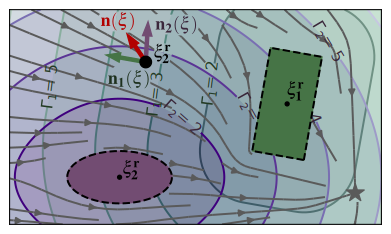
\includegraphics[width=0.5\textwidth]{figures/normal_and_gamma_field_visualization_annotated.pdf}}
\caption{
The $\Gamma$-field is defined individually for each of the obstacles. At each position $\vecs \xi$, we can evaluate the surface normals $\vect n(\vecs \xi)$. 
The desired velocity $\vect f(\vecs \xi)$ (gray) is avoiding collision with the obstacles and converges towards the attractor (black star).}
\label{fig:resultant_normal}
\end{figure}

\subsection{Force Control}

\subsubsection{Rigid Body Dynamics}
A physical system requires an interaction force that moves it around. Hence, general second-order dynamical equations are given by:
\begin{equation}
\matd{M}(\vecs\xi)\vecs{\ddot\xi} + \matd{C}(\vecs\xi, \vecs{\dot\xi})\vecs{\dot\xi} + \vect g(\vecs\xi) = \vecs{\tau_c} + \vecs{\tau_e}
 \label{eq:robot_dynamics}
\end{equation}
where we have the mass matrix of the robot $\matd M(\vecs\xi) \in \mathbb{R}^{N \times N}$, the Coriolis matrix $\matd C(\vecs\xi,\vecs{\dot\xi}) \in \mathbb{R}^N$, the gravity vector $\vect g(\vecs\xi) \in \mathbb{R}^N)$, the control torque $\vecs{\tau_c} \in \mathbb{R}^N$, and the external torque, also referred as disturbance, $\vecs{\tau_e} \in \mathbb{R}^N$.

\subsubsection{Passive Control}
Passive interaction control \cite{kronander2015passive} offers a powerful method for computing control forces from a velocity vector field. This controller provides selective disturbance rejection based on the direction of motion. Typically, the controller is configured with high damping along the direction of motion, ensuring rapid convergence of the robot's velocity to the desired value and thereby achieving excellent tracking performance. In contrast, the controller exhibits high compliance in the direction perpendicular to the motion, enabling flexible behavior and greater resistance to external forces. This versatile approach enables robots to adeptly navigate dynamic environments while maintaining stable and precise control, making it a valuable asset for a wide range of robotic applications.
% Passive interaction control \cite{kronander2015passive} enables computing a control force from a velocity vector field. The controller allows selective disturbances rejection, given the direction of motion. Most commonly, the controller is set to have high damping in the direction of the motion but be compliant in the direction perpendicular to the motion. High damping implies results in the robot's velocity rapidly converging to the desired velocity, leading to good tracking performance. Conversely, high compliance results in flexible behavior and resist little to external forces.

The passive control force \cite{kronander2015passive} is given as:
\begin{equation}
	\vecs{\tau_c} = \vect g (\vecs\xi) 
	% + \matd{D}(\vect \xi, \dot{\vect \xi}) \dot{\vect \xi}  
	+ \matd{D}(\vecs\xi) \left(\vecs f(\vecs\xi) - \vecs{\dot\xi} \right) 
\label{eq:control_command}
\end{equation}
This control law embeds a gravity compensation term and a damping term, which decreases the difference between the desired velocity $\vecs f(\vecs\xi)$ and the actual velocity $\vecs{\dot\xi}$.

The positive definitie damping matrix $\matd D(\vecs\xi) \in \mathbb{R}^{N \times N}$ is designed to allow for damping in each sub-direction:
\begin{equation}
   \matd {D}(\vecs \xi) = \matd{Q}(\vecs\xi)\matd{S}(\vecs\xi) \matd{Q} (\vecs \xi)^{-1}
\label{eq:damping_matrix}
\end{equation}
where $\matd Q(\vecs \xi) \in \mathbb{R}^{N \times N}$ is an othonormal basis matrix. 
formed by $\vecs{q}_1, \vecs q_2, ..., \vecs q_N$ The first vector is pointing in the desired direction of motion: $\vecs q_1 = \dot{\vecs \xi} / \lVert \dot{\vecs \xi} \rVert$.

The diagonal matrix $\matd{S}(\vecs\xi) \in \mathbb{R}^{N \times N}$ consists of damping factors in the corresponding direction.
Increase consistency with the desired velocity s achieved, by setting the first damping factor $s_1 \geq 0$ to a high value. The damping in the remaining directions $s_i \geq 0$ with $i = 2 .. N$ is set lower to allow compliance perpendicular to the motion. 

\subsection{Stability Analysis} \label{sec:trad_passive}
It is crucial to consider varying control parameters carefully, as they can inject energy into a system, potentially leading to unstable behavior \cite{ferraguti2013tank}. Ensuring stability guarantees is of paramount importance to safeguard both the hardware and the environment in which the control system operates.

In human-robot interaction, the robot faces external disturbances of unknown nature. To achieve stable and bounded behavior in the face of such disturbances, \textit{passivity} analysis proves to be a valuable tool. By employing passivity analysis, the control system can be designed to maintain stable responses (bounded system) in the presence of any external force (bounded input). This property enhances the reliability and safety of the control system, making it more resilient in dynamic and uncertain environments.

\begin{definition}[Passivity \cite{willems1972dissipative, sepulchre2012constructive}] \label{def:passivity}
	A dynamical system with input $ u \in \mathcal{U}$ and output $y \in \mathcal{Y}$ is passive with respect to the supply rate $s : \mathcal{U} \times \mathcal{Y} \rightarrow{R}$ if, for any $u: \mathbb{R}_{>0} \rightarrow \mathcal{U}$ and any time $t^* \geq 0$ the following is satisfied
  \begin{equation}
	  \int_0^{t^*} s \left( u(t),  y (t) \right) d \tau \geq S(t^*) - S(0) 
  \end{equation}
  where $S(t) \in \mathbb{R}_{\geq 0}$ is the storage function.
\end{definition}

Since two passive systems result in a passive system \cite{sepulchre2012constructive}, by ensuring that a controller is passive it follows that its interaction with its (passive) environment results in a passive system.

\subsection{Problem Statement}
Following assumptions are made about the desired velocity $\vecs f(\vecs\xi)$:
\begin{enumerate}
    \item $\vecs f(\vecs\xi)$ is continuous for all reachable states.
    %% \item $\vecs f(\vecs\xi)$ has a single equilibrium point $\vecs\xi^a$, such that $\{ \vecs \xi : \vecs f(\vecs \xi) = \vecs 0 \} = \{ \vecs\xi^a \}$. 
    \item $\vecs f(\vecs\xi)$ is bounded, i.e., there exists a constant $v^{\mathrm{max}} \in \mathbb{R}$ such that $\| \vecs f(\vecs\xi) \| \leq v^{\mathrm{max}} \;\; \forall \, \vecs \xi \in \mathbb{R}^N$
    \item $\vecs f(\vecs\xi)$ leads to a collision-free motion, i.e., $\vecs{n_o}(\vecs\xi)^T \vecs f(\vecs\xi) \geq 0$ as $\Gamma_o(\vecs \xi) \rightarrow 1 \quad \forall o = 1 .. N^{\mathrm{o}}$ with the normal $\vecs n_o$ and distance $\Gamma_o$ of the $o$-th obstacle. 
\end{enumerate}

Note that velocity obtained using the obstacle avoidance method described in \eqref{eq:modulated_ds}, fulfills these conditions if base velocity $\vecs f^b(\vecs \xi)$ is continuous and bounded.


\section{Obstacle Aware Passivity} \label{sec:obstacle_aware_passivity}
We propose a novel controller, which ensures passivity as defined in \eqref{eq:control_command} but adapts the damping matrix given in \eqref{eq:damping_matrix} based on the desired velocity $\dot{\vecs \xi}$ and obstacles in the surrounding. 
Hence, the damping matrix smoothly changes from being aligned with the direction of the velocity, as used in \cite{kronander2015passive}, to be aligned with the averaged normal of the obstacles.
Far away the system is designed to follow the initial velocity, but when approaching the obstacle, it increases the damping, which decreases the chance of a collision.

The desired damping matrix transitions smoothly between two states: velocity preserving, and collision avoidance. It is defined as a linear combination:
\begin{equation}
    \matd D(\vecs\xi) = \left(1 - w(\vecs\xi) \right) {\matd D^{f}}(\vecs\xi) + w(\vecs\xi)  {\matd D^{\mathrm{obs}}}(\vecs\xi) \label{eq:damping_summation}
\end{equation}

The danger $w(\vecs\xi) \in [0, 1]$ indicates the proximity to the obstacles based on the distance function $\Gamma_o(\vecs \xi)$. Far away from obstacles the weight reaches $w(\vecs \xi) = 0$, whereas $w(\vecs \xi) = 1$ when approaching a boundary:
\begin{equation}
  \begin{split}
w(\vecs\xi) =
\max \left(0,  \frac{\Gamma^{\mathrm{crit}} - \Gamma(\vecs\xi)}{\Gamma^{\mathrm{crit}} - 1} \right) \| \vecs n(\vecs \xi) \| \\
\text{with} \quad
\Gamma(\vecs\xi) = \min_{o = 1..N^{\mathrm{obs}}} \Gamma_o(\vecs\xi)
\label{eq:weight_function}
\end{split}
\end{equation}
The critical distance $\Gamma^{\mathrm{crit}} \in \mathbb{R}$ defines the distance where the system has higher damping towards the obstacle.

Note that, since ${\matd D^f}(\vecs\xi)$ and $\matd {D^{\mathrm{obs}}}(\vecs\xi)$ follow design given in \eqref{eq:damping_matrix} and are positive semi-definite matrices, thus $\matd {D}(\vecs\xi)$ is positive semi-definite, too.

\begin{figure}
  \center
  \includesvg[width=0.7\columnwidth]{figures/damping_basis_construction.svg}
\caption{The damping matrix enforcing desired velocity following $\matd{D}^{f}$ has the first basis vector $\vect q_1^{f}$ which follows the avoidance velocity $\vect f(\vecs \xi)$ and damping to enforce collision avoidance with $\matd{D}^{\mathrm{obs}}$ uses the normal $\vect n(\vecs \xi)$ to construct the first direction of the decomposition basis $\vect q^{\mathrm{obs}}_1$.}
\label{fig:damping_basis_construction}
%% \label{fig_basis_3D_DS_obs}
\end{figure}

\subsection{Collision Repulsion Damping} \label{sec:obstacle_repulsion}

\subsubsection{Normal Direction}
The damping matrix $\matd D^{\mathrm{obs}}(\vecs \xi)$ rejects velocities in the direction of the obstacles. To allow this, we introduce an average normal direction:
\begin{equation}
  \vecs n(\vecs\xi) = \sum_{o=1}^{N^{\mathrm{obs}}} \vecs{n_o}(\vecs\xi)
  \frac{1 / (\Gamma_o(\vecs \xi) - 1)}{\sum_{p=1}^{N^\mathrm{obs}} 1 / (\Gamma_p(\vecs \xi) - 1)}
  \label{eq:averaged_normal}
\end{equation}
 where the unit normals $\vecs{n_o} (\vecs\xi)$  are pointing away from the obstacle $o = 1,  ..,  N^{\mathrm{obs}}$, see Figure~\ref{fig:resultant_normal}. 

The averaged normal $\vecs n(\vecs \xi)$ is a weighted linear combination of the obstacles' normals, giving more importance to closer obstacles.
Additionally, the averaged normal converges to an obstacle normal as we converge towards it, i.e., $\lim_{\Gamma_o(\vecs \xi) \rightarrow 1} \vecs n(\vecs \xi) = \vecs n_o(\vecs \xi)$.
Note that the averaged normal is a zero-vector when two obstacles oppose each other. This case will be further discussed in the next section.

\subsubsection{Decomposition Matrix}
The decomposition matrix $\matd Q^{\mathrm{obs}}(\vecs \xi)$ has its first vector aligned with the normal to the obstacle:  $\vecs q_1^{\mathrm{obs}}(\vecs\xi) =  \vecs n(\vecs\xi) / \lVert\vecs n(\vecs\xi)\rVert$ 

The second vector is set to be aligned with the desired velocity as much as possible, this will allow increased velocity following (Fig.~\ref{fig:damping_basis_construction}). However, it has to remain orthonormal to $\vect q_1^{\mathrm{obs}}$
\begin{equation}
  \vecs q_2^{\mathrm{obs}} = \frac{\hat{\vecs q}_2^{\mathrm{obs}}}{\| \hat{\vecs q}_2^{\mathrm{obs}} \|}
  \quad
  \hat{\vecs q}_2^{\mathrm{obs}} = \vecs q_1^{f} - \vecs q_1^{\mathrm{obs}} p \quad  \forall \, \vecs \xi : | p | < 1
\end{equation}
where the object weight is given as $p = \dotprod{\vecs q_1^{\mathrm{obs}}}{\vecs q_1^{f}}$
For the case that $| p | = 1$, the second basis $\vecs q_2^{\mathrm{obs}}$ is set to be any orthonormal vector. The remaining vectors $\vecs q_i^{\mathrm{obs}}, i = 3, .., N$ are constructed to form an orthonormal basis to the first two.

\subsubsection{Damping Values}
Analogously, we smoothly define the values of the diagonal matrix $\matd{S}^{\mathrm{obs}}(\vecs \xi)$:
\begin{equation}
  \matd{S}_d^{\mathrm{obs}}(\vecs \xi) =
  \begin{cases}
    s^{\mathrm{obs}} & d = 1 \\
    | p | s^c + (1 - | p |) s^{f} & d = 2 \\
    s^c & d \geq 3 
  \end{cases}
  \quad d = 1 .. N\
\end{equation}
where the damping along the nominal direction $s^{f} \in \mathbb{R}$, obstacle-damping $s^{\mathrm{obs}} \in \mathbb{R}$, and the compliant-damping $s^c \in \mathbb{R}$ are user-defined parameters which define the behavior of the passive-controller.

The first entry of $\matr{S}^{\mathrm{obs}}$ indicates the damping towards the obstacle, and the second entry indicates the desired velocity following. Note how the later value decrease, when normal and velocity are becoming parallel.

\subsubsection{Damping Only Towards Obstacle} \label{sec:damping_only_toward}
To reject only the disturbances that push the agent against the obstacle and allow compliance away from the obstacle, we have added a new feature. Hence, in case the robot is already moving away, i.e., $\vecs{\dot\xi}^T \vecs n(\vecs\xi) > 0$,  the value of $\matd{S}^{\mathrm{obs}}_1$ gets overwritten with $s^{c}$, the general, compliant damping value:
\begin{equation}
  \matd{S}_1^{\mathrm{obs}} =
  \begin{cases}
    s^{\mathrm{obs}} & \text{if} \;\; \left(\vect f(\vecs \xi) - \vecs{\dot \xi} \right)^T \vecs n(\vect \xi) > 0 \\
    s^{\mathrm{c}} & \text{otherwise}
  \end{cases}
  \label{eq:leaving_compliance}
\end{equation}
This ensures that the agent can move freely away from the obstacle, but is damped when pushed towards.


\subsection{Velocity Preserving Damping}
The decomposition matrix $\matd Q^{f}$ is an orthonormal basis with the first vector being parallel to the desired velocity $\vect f(\vecs\xi)$. Let us define $\vecs q^{f}_1 (\vecs\xi) = \vect f({\vecs \xi}) / \lVert \vect f({\vecs \xi}) \rVert$, as proposed in Section~\ref{sec:trad_passive}. Hence, the values of the diagonal matrix $\matd S^{f}$ are high in the direction of the desired velocity (first component), but more compliant in the remaining directions. 
However, we need to additionally ensure that when moving in a narrow passage between two obstacles, where the normal vector cancels $\vect n(\vecs \xi) \approx 0\vect 0$, but a low distance value $\Gamma(\vecs \xi) \approx 1$, the damping perpendicular to the velocity direction is high. Hence, we propose:
\begin{equation}
  \begin{split}
  \matd{S}^{f}_{d} =
  \begin{cases}
    s^{f} & d = 1 \\
    w^p s^{\mathrm{obs}} + (1- w^p) s^s & d \geq 2 
  \end{cases} \quad d = 1 .. N\\
  \text{with} \quad
  %w^p = \min \left(1,  \| \vecs n(\vecs \xi) \|^2 + \left(\frac{\Gamma(\vecs \xi) -1}{\Gamma^{\mathrm{crit}} - 1}\right) ^2 \right)
   w^p = \min \left(1,  \| \vecs n(\vecs \xi) \|^2 + \left(\frac{\Gamma^{\mathrm{crit}} -\Gamma(\vecs \xi)}{\Gamma^{\mathrm{crit}} - 1}\right) ^2 \right)
  \end{split}
\end{equation}

\subsection{Damping Parameter Design}
In general, higher values result in improved velocity following and disturbance repulsion, whereas lower values allow more compliant behavior.

The damping value in the direction of the obstacle is set high $s^{\mathrm{obs}}$ to ensure obstacle avoidance with any possible disturbance. 
Conversely, the damping in the direction of the velocity $s^{f}$ is set medium to high, as the system should follow the desired velocity $\vect f(\vecs \xi)$, however, it should still remain compliant if needed.
Finally, for all other directions, a low damping value $s^{c}$ should be chosen to facilitate interaction.
This can be summarized as:
\begin{equation}
s^{\mathrm{obs}} > s^{f} \gg s^{c} > 0
\end{equation}

\subsection{Passivity Analysis}
The stability analysis of the system gives information about the region of stability of the proposed controller. The passivity is analyzed by observing the evolution of the kinetic energy of the system, which is given as:
\begin{equation}
	W(\vecs \xi, \vecs{\dot \xi}) = \frac{1}{2}  \dot{\vecs{\xi}}^T \matd{M}(\vecs \xi) \dot{\vecs{\xi}} \label{eq:energy_system}
\end{equation}

\begin{lemma} \label{lemma:passivity}
  % Let $\vect f(\vecs \xi)$ be the desired velocity with bounded magnitude, i.e., $\| \vect f(\xi) \| < \infty, \forall \xi \in \mathbb{R}^N$.
   Let us assume a robotic system as described in \eqref{eq:robot_dynamics} is controlled using \eqref{eq:control_command} using the damping matrix $\matd D(\vecs \xi)$ given in \eqref{eq:damping_summation} with damping values $s_i = 1$.
   The system is passive with respect to the input-output pair $\vecs \xi_e$, $\vecs{\dot \xi}$ when exceeding the desired velocity $\vect f(\vecs \xi)$ , i.e., $\dot{W} \leq \vecs{\dot \xi}^T \vecs \tau^e, \; \forall \vecs \xi \in \mathbb{R}^N: \| \vecs{\dot \xi} \| \geq \| \vect f(\vecs \xi) \|$ and the storage function being the kinetic energy $W \in \mathbb{R}$ given in \eqref{eq:energy_system}
\end{lemma}

\begin{proof}
The time derivative of storage function $W$ can be evaluated as:
\begin{align}
  % \begin{split}
    \dot W(\vecs \xi, \vecs{\dot \xi}) &=
    \vecs{\dot \xi}^T \matd M(\vecs \xi) \vecs{\ddot \xi}  + \frac{1}{2} \vecs{\dot \xi}^T \dot{\matd M}(\vecs \xi) \vecs{\dot \xi}  \nonumber \\
  &= \frac{1}{2} \vecs{\dot \xi}^T \left( \dot{\matd M}(\vecs \xi) - 2 \matd C(\vecs \xi) \right) \dot{\vecs \xi} - \vecs{\dot \xi}^T \matd{D}(\vecs \xi) \vecs{\dot \xi} + \vecs{\dot \xi}^T \vecs \tau^e \nonumber \\
  &= - \vecs{\dot \xi}^T \matd{D}(\vecs \xi) \left( \vecs{\dot\xi} - \mathbf{f}(\vecs \xi) \right) + \vecs{\dot\xi}^T \tau^e
  % \end{split}
\end{align}
where we use the fact that $\dot{\matd M} - 2 \matd C$ is skew-symmetric, and hence the corresponding summand is zero.

% \subsubsection{Stability with Uniform Damping}
Let us investigate the region where the passivity holds. From the Lemma, we assume that all damping values are equal to one, hence we have:
\begin{equation}
	\matd{D}({\vecs \xi}) = \matd{Q}({\vecs \xi}) \matd{S} ({\vecs \xi}) \matd{Q}({\vecs \xi})^{-1}= \matd{Q}({\vecs \xi}) \matd{I} \matd{Q}({\vecs \xi})^{-1} = \matd{I}
\end{equation}
where $\matd{I}$ is the identity matrix.

It follows that the system is passive with respect to the input, the external force $\tau^e$, and the output, the velocity $\dot {\vecs \xi}$, as long as:
\begin{equation}
	\dot{\boldsymbol {\vecs \xi}}^T \matd{D}({\vecs \xi}) \left(\dot{\boldsymbol {\vecs \xi}} - \boldsymbol{f}(\boldsymbol {\vecs \xi}) \right) = 
    \dot{{\vecs \xi}} ^ T \Delta \vect{f}  \geq 0 
 \; , \quad
 \Delta \mathbf{f} = \dot{{\vecs \xi}} - \mathbf{f}({\vecs \xi})
\end{equation}

On the border of this region, the two vectors $\Delta \mathbf{f}$ and $\dot{\mathbf {\vecs \xi}}$ are orthogonal.
Hence using Thale's theorem, this region can be evaluated as a circle with radius $\| \mathbf{f} ({\vecs \xi}) \| / 2$ and center $\mathbf{f}(\mathbf {\vecs \xi}) / 2$, as visualized in Figure~\ref{fig:passivity_analysis}.

Moreover, the system is passive as long as the observed velocity $\dot{{\vecs \xi}}$ is outside the circular-red region, which is a subset of the region where the magnitude of the observed velocity is smaller than the desired velocity $\mathbf{f}({\vecs \xi})$, i.e.,
\begin{equation}
	\dot W({\vecs \xi}, \dot{{\vecs \xi}}) \leq \dot{{\vecs \xi}}^T \vecs \tau^e
 \quad \forall {\vecs \xi} : \| \dot{{\vecs \xi}} \| \geq\| \mathbf{f}({\vecs \xi}) \| 
\end{equation}

\begin{figure}[b]
	\centering
	% \includesvg[width=0.7\columnwidth]{figures/passivity_analysis.svg}
    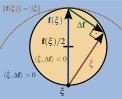
\includegraphics[width=0.7\columnwidth]{figures/passivity_analysis}
	\caption{The system is passive velocities $\dot{\vecs \xi}$ which are larger than the desired velocity $\vect f(\vecs \xi)$, i.e., outside the dashed orange circle.
    However, the system can be non-passive for small velocities when  $\dotprod{\dot{\vecs \xi}}{\Delta \vect f} < 0$ (yellow circle). }
	\label{fig:passivity_analysis}
\end{figure}

\end{proof}

As in the red region, the system is not passive; the storage function $W$ could increase, and hence the velocity $\dot {\vecs \xi}$ could increase in a non-passive manner. This behavior is not unexpected, as the controller is designed to approach a desired DS $\vect{f}({\vecs \xi})$. Hence, as long as the desired velocity is not reached, the kinetic energy increases even with no force input $\vecs \tau^e$. While the passivity in Lemma~\ref{lemma:passivity}, only holds in a certain region. We can use this property to ensure the stability of the system:

\begin{theorem}  \label{theorem:passivity}
  Let $\vect f(\xi)$ is the desired velocity $\vect f(\vecs\xi)$ with bounded magnitude, i.e., $\| \vect f(\xi) \| < v^{\mathrm{max}}, \forall \xi \in \mathbb{R}^N$.
   The closed loop system \eqref{eq:robot_dynamics} is bounded-input, bounded-output (BIBO) stable using the controller from \eqref{eq:control_command} and damping matrix $\matd D(\vecs \xi)$ given in \eqref{eq:damping_summation} with respect to the input disturbance forces $\vect \tau^e$, and output the velocity $\dot{\vecs \xi}$.
\end{theorem}
 
\begin{proof}
From Lemma~\ref{lemma:passivity}, the system is passive when the magnitude of the velocity is larger than the dynamics, i.e. $\| \dot{\vecs \xi} \| > \|\vect f(\vecs \xi) \|$, the orange circle in Figure~\ref{fig:passivity_analysis}.
Inside this region, the system is not passive, and the velocity $\dot {\vecs \xi}$ can increase. However, the velocity increase is limited to staying below $\| \vect f({\vecs \xi}) \|$ before the system enters the region where it is passive. Hence, the control cannot introduce unexpected energy.
It follows that the system has a bounded output as long as the desired velocity $\mathbf{f}({\vecs \xi})$ is stable and the input $\int_{0}^T \dot{{\vecs \xi}}^T \vecs \tau^e dt$ is bounded. 
% Since as soon as the observed velocity $\| \dot{{\vecs \xi}} \| $ is larger than the desired velocity, the system behaves passively. Hence, the control cannot introduce unexpected energy.

% \subsubsection{Stability with General Damping}
From \eqref{eq:damping_summation}, a general damping matrix $\matd{S}(\vecs \xi)$ has non-uniform values. Hence, the analysis needs to be extended to general values.
The damping matrix $\matd{D}({\vecs \xi}) = \matd{Q}({\vecs \xi}) \matd{S}({\vecs \xi}) \matd{Q}({\vecs \xi})^{-1}$, can be interpreted as a coordinate transfer, such that:
\begin{equation}
	\vecs{\bar v} = \sqrt{\matd{S}({\vecs \xi})} \matd{Q}({\vecs \xi})^{-1} \dot{{\vecs \xi}}
	\quad \text{and} \quad
	\bar{\Delta \mathbf f} = \sqrt{\matd{S}({\vecs \xi})} \matd{Q}({\vecs \xi})^{-1} \Delta \mathbf{f}
\end{equation}
where the square root of the diagonal matrix $\Lambda({\vecs \xi})$ is taken element-wise:
\begin{equation}
\dot{\vecs \xi}^T \matd{D}({\vecs \xi}) \Delta \mathbf{f} = \vecs{\dot \xi}^T \matd{Q}({\vecs \xi}) \matd{S}({\vecs \xi}) \matd{Q}({\vecs \xi})^{-1} \Delta \mathbf{f} = \vecs{\bar v}^T \bar{\Delta \mathbf f}
\end{equation}
The analysis described in Fig.~\ref{fig:passivity_analysis} can hence be applied in the transformed space, too. 

For an orthogonal decomposition matrix $\matd{Q}(\boldsymbol{{\vecs \xi}})$, the region of non-passivity is an ellipse where the direction of the axes points along column vectors of $\matd{Q}({\vecs \xi})$, and the corresponding axes lengths are the diagonal elements of $\| \mathbf{f}({\vecs \xi})^T \sqrt{\matd{S}({\vecs \xi})}\| / 2 \sqrt{\matd{S}({\vecs \xi})}^{(-1)}$. 

If the axes' lengths are large, this can lead to accelerating the velocity even though it is already larger (but not pointing in the correct direction) than the desired velocity. However, the non-passive region is still bounded by an ellipse, and hence a maximum velocity.

While the passivity statement of Lemma~\ref{lemma:passivity} is local only, hence the controller can introduce energy into the system outside of the passive region. However, in such a case the system the velocity of the system increases and the system will enter the passive region system since it is bounded by a velocity limit.
However, passivity is used to prove that a controller does not \textit{pump} energy In that case, the controller acts passive and is ensured not to increase the system's energy anymore.
\end{proof}

This proof extends to a basis $\matd{Q}$, which is not orthogonal. However, in such a case, the controller must be carefully chosen to ensure that the speed up is limited when the basis is close to singular, for example by limiting the relative difference of the stretching vectors.

As stable behavior is ensured for a general shape of a damping matrix $\matd{D}$, the global stability proof extends to the general passive interaction control introduced in \cite{kronander2015passive}.

% Note, that in the case of $\langle e_2, e_n \rangle \neq 0$ the choice of $e_2$ does not matter as the corresponding  weight from \eqref{eq:eig2_weight} is $w_2 = 0$, hence it $\lambda_2 = \lambda$, as all eigenvalues.

\section{Collision Avoidance} \label{sec:collision_avoidance}

% \subsection{Disturbance Repulsion}
The fundamental requirement of the proposed controller is its ability to ensure collision avoidance in the presence of external disturbances.
as the damping as proposed in \eqref{eq:control_command} does not explicitly consider external forces. Rather, the force accelerate the robot and hence results in a deviating velocity $\dot{\vecs \xi}$. Which is finally observed the controller, and corrected to approach the desired velocity $\ddot{\vecs \xi}$.\footnote{Note, that for a discrete time (digital) controller, this results in a delay.}

We further look at impact which happen during a short time period $\Delta t \ll 1$ during which a force is applied. Hence, hence we assume the velocity after impact $\vect v^I$:
\begin{align}
	 % \begin{split}
	\vect v^I
	  \approx \int_{t^I}^{t^I + \Delta t} \ddot{\vecs \xi} dt  
	  \approx \int_{t^I}^{t^I + \Delta t} \matd{M}^{-1}(\vecs \xi)  \vecs \tau_e \, dt  
	 % \end{split}
	  \label{eq:impact_velocity}
\end{align}
using the controller from \eqref{eq:robot_dynamics}, and under absence of the control force $\vecs \tau_c$ during this short timeframe. Additionally, $\{\vect \xi \}_{t^I}$ is the velocity before the impact.
 
% Since the magnitude of the normal is limited to $1$, the control weight is limited as: 
% \begin{equation}
% w(\vecs \xi) \geq \frac{\Gamma^{\mathrm{crit}} - \Gamma(\vecs \xi)}{\Gamma^{\mathrm{crit}} - 1}
% \end{equation}
% under the assumption that $\Gamma^{\mathrm{crit}} \geq 1$.

% Using the controller design from \eqref{eq:control_command} the velocity can be computed as:
% \begin{equation}
% \begin{split}
% 	\{ \vecs{\dot \xi} \}_{t} 
% 	& = \int \vecs{\ddot \xi} \, dt = \int \matd{M}^{-1} \matd{D}  \bigl( \vecs{\dot \xi} - \vecs f(\vecs \xi) \bigr) \, dt \\
% 	& = \int \matd{M}^{-1} \matd{D} \bigl( \vecs{\dot \xi} - \vecs f(\vecs \xi) \bigr) \, dt \\
% 	& = \matd{M}^{-1} \int \left( (1 - w) \matd{D}^f + w \matd{D}^{o} \right)  \bigl( \dot{\vecs \xi} - \vecs f(\vecs \xi) \bigr) dt\\
% 	& = \matd{M}^{-1} \int  \matd{D}\bigl( \vecs \xi - t \vecs f(\vecs \xi) \bigr) + C_t \\
% 	% &  \underset{}\{ {\vecs \xi} \}_0 = \vecs f(\vecs \xi) + \vecs v^I{=} \matd{M}^{-1} \matd{D}  \left( \xi - t \vecs f(\vecs \xi) \right) + C_t \\
% 	&  = \matd{M}^{-1} \matd{D}  \bigl( \vecs \xi - \{\vecs \xi\}_0  - t \vecs f(\vecs \xi) \bigr) + \vecs f(\vecs \xi) + \vecs v^I \\
%     % & \approx \int \matd{M}^{-1} \matd{D} \vect f(\vecs \xi) \, dt
% \end{split}
% \label{eq:velocity_evolution}
% \end{equation}
% using $\{ {\vecs \xi} \}_0 = \vecs f(\vecs \xi) + \vecs v^I$ to find the integration constant $C_t$.

Let us assume the desired velocity $\vect f(\vecs \xi)$ is a constant, collision free vector field which is constant and parallel to the surface to a flat surface (see Fig.~\ref{fig:disturbance_with_parallel_velocity}):
\begin{equation}
	\dotprod{\vect f(\vecs \xi)}{\vecs n(\vecs \xi)} = 0
	 \qquad
\vect f(\vecs \xi) = \text{const.}
\, , \;
\vect n(\vecs \xi) = \text{const.}
\label{eq:parallel_velocity}
\end{equation}
where $\vecs n(\vecs \xi)$ is the normal vector of the surface. 

\begin{lemma} \label{lemma:damping_collision_avoidance}
	A point like agent evolves according to the dynamical system evolves with the rigid body dynamics given in \eqref{eq:robot_dynamics} controlled by \eqref{eq:control_command}, with damping matrix $\matd{D}$ from \eqref{eq:damping_summation}, and a negligible Coriolis effect.
	A motion starting in free space remains collision-free for all times, i.e., $\Gamma( \{\vecs \xi_t\}) \geq 1$ with $t \geq 0$ if the impact velocity $v^I$ as given in \eqref{eq:impact_velocity} at time $t=0$ is limited by $\| \vect v^I\| < s^{\mathrm{f}} \| \vecs \xi - \vecs \xi^b \| / m$, with respect to the closest surface point $\vecs \xi^b \in \mathbb{R}^N$ and mass $m \in \mathbb{R}_{>0}$.
\end{lemma}

% \begin{lemma}
% 	A dynamical system evolves with the rigid body dynamics given in \eqref{eq:robot_dynamics} controlled by \eqref{eq:control_command}, with damping matrix $\matd{D}$ from \eqref{eq:damping_summation}, and a negligible Coriolis effect.
%     A point-like agent starting at position $\vect p = \{{\vecs \xi}\}_0$ close to the surface, i.e., $\Gamma( \vect p) \approx 1$ is guided by a velocity field $\vect f(\vecs \xi)$ parallel to the surface with a starting velocity $\vect v^0= \vect f(\{{\vecs \xi}\}_0)$.
%     A large disturbance towards the obstacle results in a velocity of $\{\dot{\vecs \xi}\}_0 = \vect v^I +  \vect v^0$ after the impact, with $\| \vect v^I \| \gg \| \vect v^0 \|$.
% 	A motion starting in free space remains collision-free for all times, i.e., $\Gamma( \{\vecs \xi_t\}) \geq 1$ with $t \geq 0$ if the impact velocity is limited by $\| \vect v^I\| < s^{\mathrm{o}} \| \vecs \xi - \vecs \xi^b \| / m^{\mathrm{min}}$, with respect to the closes surface point $\vecs \xi^b \in \mathbb{R}^N$ and mass $m \in \mathbb{R}_{>0}$.
% \end{lemma}

\begin{proof}

an environment where the robot should just rest, hence the desired velocity field is :
\begin{equation}
\begin{split}
	\{ \vecs{\dot \xi} \}_{T} 
	& = \int \vecs{\ddot \xi} \, dt = \int \matd{M}^{-1} \matd{D} \left( \vecs{\dot \xi} - \vect f(\vecs \xi ) \right) \, dt \\
	& = \matd{M}^{-1} \int \left( (1 - w) \matd{D}^f + w \matd{D}^{o} \right) \left( \vecs{\dot \xi} - \vect f (\vecs \xi ) \right) dt \\
	\end{split}
\label{eq:velocity_evolution}
\end{equation}

From \eqref{eq:parallel_velocity}, the vector field is constant, and the surface does not have any curvature, it follows from \eqref{eq:damping_summation} that the damping matrices $\matd{D}^o$ and $\matd{D}^f$ are constant. 
Hence, we perform the integration to find the time $T$ at which the agent stop moving towards the obstacle, which will then enable us to evaluate the distance travelled as a function of the velocity after disturbance $\vect v^I$. According to the Bony-Bezis theorem \parencite{bony1969principe}, the velocity is collision-avoiding when it is zero along the normal direction:
\begin{equation}
	\left| \vect n(\vecs \xi)^T \, \{ \vecs{\dot \xi} \}_{t} \right| = 0
\end{equation}

Thus in the following analysis, we focus on the normal component of the vectors only. Thus, in the rest of this paragraph, the component along the normal will simply be denoted by scalar values, e.g. $\xi = \dotprod{\vecs \xi}{\vecs n(\vecs \xi)} \vecs n(\vecs \xi)$.
	Furthermore, by design of the damping matrixes, we know from \eqref{eq:obstacle_damping_values} 
	that $\matd{D}^o(\vecs \xi) \vect n(\vecs \xi) = s^o \vect n(\vecs \xi)$, and from \eqref{eq:velocity_damping} we know that $\matd{D}^f(\vecs \xi) \vect n(\vecs \xi) = s^f \vect n(\vecs \xi)$. Hence, we get:
\begin{align}
	0 & = \left| \vect n(\vecs \xi)^T \, \{ \vecs{\dot \xi} \}_{t} \right| 
	  = \frac 1 m \int ( (1-w) \vect n^T \matd{D}^f \vect n + w s^{o} ) \, {\dot \xi} \, dt \nonumber \\
	   & < \frac 1 m \int  s^{f}  \, {\dot \xi} \, dt 
	   = \frac{s^f}{m} (\xi - \{ \xi \}_0 ) + v^I \, dt 
\end{align}
where $m = \max{\left(\text{eig}(\matd{M})\right)}$, we additionally assume that the damping matrices are positive definite. 

The maximum displacement follows as:
\begin{equation}
	\| {\xi} - \{\xi \}_0 \| \geq \| v^I \| {m} / {s^{\mathrm{f}}} 
\end{equation}

To see when the differences reaches zero, we can compute
\begin{equation}
 \|	\{ \vecs{\dot \xi} \}_T - \vect f(\vecs \xi) \| = 0
 \quad \Rightarrow \quad
    \| \vecs{\xi}_1 -  \vect p_1 \| = \| \vecs v^I_1 \| {m} / {s^{\mathrm{o}}} 
 \end{equation}
\end{proof}

Note, that while Lemma~\ref{lemma:damping_collision_avoidance} is under the assumption of constant desired velocity and flat surface. While most desired velocity are a function of the position, and morover obstacles are finite and hence have sume surface curvature. However, since the algorithm explores the limit, hence large disturbance forces and velocities after disturbance $\| \vect v^I \| \gg 1 \|$. As a result, the distance travelled along the surface is small, and it can be considered locally flat. Additionally, in the extreme case, the disturbance happens close to the surface, and hence the desired velocity is almost constant.  

\begin{figure}[htb]
\centering
 % \begin{subfigure}{0.99\columnwidth}
  \centerline{\includegraphics[width=0.99\columnwidth]{figures/parallel_avoidance_obstacle}}
  \caption{A disturbance occurs of a point-agent at position $\vect p^0$ with velocity after the impact of $\{ \dot{\vecs \xi} \}_0 = \vect v^0 + \vect v^I$. A high damping in the direction of the obstacle in the presence of a constant velocity field (gray) ensures collision avoidance. Whereas different damping values $s^{\mathrm{o}}$ and optionally a maximum repulsion force $\vecs \tau^{\mathrm{max}}$ lead to different trajectories.}
  \label{fig:disturbance_with_parallel_velocity}
% \end{subfigure}
\end{figure}
    
\begin{proof}
Since we assume a point-like agent, the mass matrix $\matd{M}(\vecs \xi)$ is constant, with diagonal values of $m$. The damping matrix in the proximity of a single obstacle is approximated as follows:
\begin{equation}
\Gamma(\vecs \xi) \approx 1
\; \underset{\eqref{eq:averaged_normal}, \, \eqref{eq:weight_function} } {\Rightarrow} \;
\begin{array}{l}
% \lim_{\Gamma(\vecs \xi) \rightarrow 1} \| \vect n(\vecs \xi) \| = 1, \\
% \lim_{\Gamma(\vecs \xi) \rightarrow 1}\; w(\vecs \xi) = 1
\| \vect n(\vecs \xi) \| = 1 \\
w(\vecs \xi) = 1
\end{array}
% \quad 
\underset{\eqref{eq:damping_summation}} {\Rightarrow} \quad
\matd D(\vecs \xi) = \matd{D}^o(\vecs \xi)
\end{equation}

Using the controller design from \eqref{eq:control_command} the velocity can be computed as:
\begin{equation}
\begin{split}
    \vecs{\dot \xi} & = \int \vecs{\ddot \xi} \, dt 
    = \int \matd{M}^{-1} \matd{D}  \left( \vecs{\dot \xi} - \vecs f(\vecs \xi) \right) \, dt \\
    % & \approx \int \matd{M}^{-1} \matd{D} \vect f(\vecs \xi) \, dt
\end{split}
\label{eq:velocity_evolution}
\end{equation}

Due to high velocity towards the obstacle after impact, relative to tangent velocity, i.e., $\| \vect v^I \| \gg \| \vect v^0 \|$, as well as the proximity to the obstacle from $\Gamma(\vecs \xi) \approx 1$, the agent is only able to move little before having to reject the disturbance. 
As a result, we can assume that the changes of the velocity field and the obstacle curvature are negligible, and hence we have $\vect f(\vecs \xi) = \text{const.}$ and $\vect n(\vecs \xi) = \text{const.}$
Using \eqref{eq:obstacle_damping_values} results in a constant damping matrix with damping values:
\begin{equation}
    \matd{S}^o_1 = s^o
    \; , \quad
    \matd{S}^o_2 = s^f
    \; , \quad
    \matd{S}^o_d = s^c \;\;\; d = 3 .. N
\end{equation}
From \eqref{eq:first_obstacle_basis}, we know that the first decomposition vector $\vect q_1^o(\vecs \xi)$ points along the normal $\vect n(\vecs \xi)$, and the second $\vect q_2^o(\vecs \xi)$ along the desired dynamics $\vect f(\vecs \xi)$.

% This allows for the analysis of the velocity from \eqref{eq:velocity_evolution} along decomposition direction $q_d^o$. In the tangent plane, the impact did not change the velocity, and hence:
% \begin{equation}
% \begin{split}
%     \dot{\vecs \xi}_d & = \int \matd{M}^{-1} \matd{D}  \left( \vecs f_d(\vecs \xi) - \vecs f_d(\vecs \xi) \right) \, dt  =  \vect v^0_d
%     %\qquad \text{with} \quad
% \end{split}
% \end{equation}
% with $d = 2 .. N$.

The velocity in the tangent plane does not lead to any impact. Hence, we can analyse the evolution of the velocity in the direction of the normal of the obstacle $\vecs{\dot \xi}_1$:
\begin{equation}
    \vecs{\dot \xi}1 = \int \frac{s^{\mathrm{o}}}{m} \vecs{ \dot \xi}_1 \, dt = \frac{s^{\mathrm{o}}}{m} \left(\vecs{\xi}_1 - \vect p_1 \right)  + \vecs v^I_1 \label{eq:velocity_with_control}
\end{equation}
% where $m = \min \Bigl(\text{eig} \bigl(\mathcal{M} \bigr) \Bigr)$ is the smallest eigenvalue of the mass matrix. Note, that any velocity which does not point towards the surface, will not get as close to the obstacle.

This can be used to compute the position at which the velocity in the normal direction reaches zero:
\begin{equation}
    \| \vecs{\dot \xi} _1 \| = 0
    \quad \Rightarrow \quad
    \| \vecs{\xi}_1 -  \vect p_1 \| = \| \vecs v^I_1 \| {m} / {s^{\mathrm{o}}} 
\end{equation}

As long as the disturbance is limited by
\begin{equation}
    \| \vect v^I \| < s^{\mathrm{o}} \| \vecs \xi - \vecs \xi^b \| / m
\end{equation}
it will stop at the closest surface point $\vecs \xi^b \in \mathbb{R}^N$, and hence remain collision-free.
\end{proof}

Note that the analysis is done for proximity regions of the obstacle. In any case, the robot enters this proximity region before a collision can occur. Hence, the proposed analysis holds as a general collision avoidance insurance.

Similarly, while we specifically analyze disturbances along the normal of the obstacle, any velocity after the disturbance can be divided into a part towards the obstacle, and a part parallel to the surface. Where a velocity parallel to the obstacle does not pose any danger for collision.
Yet, there is no guarantee against drifting into obstacles in the presence of highly curved surfaces and velocity fields. This is further discussed during the experiments in Section~\ref{sec:position_noise}, where it is, however, observed that the increased damping towards the obstacle significantly reduces collision in such scenarios. 

% \subsection{Disturbance Repulsion with Force Limit}
All robotic systems have a maximum force that they can exert on the environment based on the motors and their geometry, $\tau_c^{\mathrm{max}} \in \mathbb{R}_{>0}$. Additionally, such force limits are often state-dependent. A limiting force decreases the impact velocity a controller can handle while ensuring collision avoidance (Fig.~\ref{fig:disturbance_with_parallel_velocity}). Nevertheless, a maximum control force can be interpreted as adapting damping, and hence, the passivity from Theorem~\ref{theorem:passivity} holds.



% \section{Discrete Time Behavior} \label{sec:discrete_time_behavior}
So far, we've considered that the system is continuous time. 
This is a reasonable assumption, if we have a high sampling time $\Delta t$, compared to the dynamics, i.e., $\| \Delta t \, \dot{\vecs \xi} \| \ll 1$.
However, any digital controller sends a discrete control signal. In order to reject the disturbances in the presence of obstacles, a high control force is exerted (while still remaining within the control robot's limits), hence $\| \Delta t \, \vecs \tau^c \| \gg 1$. 
In this case, it is crucial to analyze the discrete-time system to guarantee stability, as high damping can lead to unstable behavior, see Figure~
\ref{fig:discrete_controller_parameters_comparison}).

\begin{figure}[htb]
\centering
  \includegraphics[width=\columnwidth]{figures/discrete_controller_parameters_comparison}
  \caption{A point-like agent with an initial velocity of $\{ \dot{\vecs \xi} \}_0 = [1 \; -1]^T$ is guided by the desired velocity $\vect f(\vecs \xi) = [1, 0]^T$, and a control matrix $\matd{D}$ with damping values $s_i$ equal in all directions, where $m$ is the mass of the point-like agent. 
  Damping values above $s_i = 2.0 m / \Delta t$ lead to unstable behavior where the higher value leads to higher oscillations. Conversely, the lowest value leads to more deviation from the straight trajectory resulting from the higher impedance. The critical value of $s_i = 2.0 m / \Delta t$ results in stable behavior with immediate correction to the desired velocity.}
  \label{fig:discrete_controller_parameters_comparison}
\end{figure}

For the discrete-time system, the position and velocity of the agent evolve as follows:
\begin{equation}
	\begin{bmatrix}
	 \vecs \xi_{t+1} \\ \dot{\vecs \xi}_{t+1}
	\end{bmatrix}
	=
	\begin{bmatrix}
	 \vecs \xi_{t} \\ \dot{\vecs \xi}_{t}
	\end{bmatrix}
	+ 
	\Delta t 
	\begin{bmatrix}
		\dot{\vecs \xi}_{t} \\ \ddot{\vecs \xi}_t 
	\end{bmatrix}
	\label{eq:discrete_time_dynamics}
\end{equation}

\begin{lemma}
	Let us consider a discrete-time system with state defined in Eq.~\eqref{eq:discrete_time_dynamics}, and is governed by the controller from Eq.~\eqref{eq:control_command} and damping matrix $\matd{D}$ defined in Eq.~\eqref{eq:damping_summation}.
	Let us consider the input the desired velocity $\vect f(\vecs \xi)$ and as output the agent's velocity $\dot{\vecs \xi}$. 
	The system is BIBO (bounded-input, bounded-stable) with respect to the velocity, i.e., $\lim_{t \rightarrow \infty} \| \dot{\vect \xi} \| < \infty$, if all eigenvalues of $\matd{M}^{-1} \matd{D}$ are less or equal to $2 / \Delta t$.
\end{lemma}

\begin{proof}
Hence, for the evaluation in discrete time, the evolution of the velocity is given by:
\begin{equation}
	\begin{split}
	& \begin{bmatrix}
	 \vecs \xi_{t+1} \\ \dot{\vecs \xi}_{t+1}
	\end{bmatrix}
	=
	\begin{bmatrix}
		\vect \xi_t + \Delta t  \; \dot{\vect \xi}_t \\ \
		\dot{\vecs \xi}_t + \Delta t \, \matd{M}^{-1} \left( \matd{D} \left( \vect f(\vecs \xi_t) - \dot{\vecs \xi}_t \right) - \matr C \right)
	\end{bmatrix} \\
	&  = %\approx
	\begin{bmatrix}
		\mathcal{I} & \mathcal{I} \Delta t \\
		\vect{0} & \mathcal{I} - \Delta t \matd{M}^{-1} \matd D 
	\end{bmatrix}
	\begin{bmatrix}
		\vect \xi_t \\ \dot{\vect \xi}_t
	\end{bmatrix}
	+ \begin{bmatrix}
		\vect{0} \\ 
		\Delta t \, \matd{M}^{-1} \matd{D} 
	\end{bmatrix}
	\hat{\vect f}(\vecs \xi_t) 
	% & \approx 
	% \begin{bmatrix}
	% 	1 & \Delta t \\
	% 	\Delta t \matd{M}^{-1} \matd D \frac{\partial \vect f}{\partial \vecs \xi} & 1 - \Delta t \matd{M}^{-1} \matd D 
	% \end{bmatrix}
	% \begin{bmatrix}
	% 	\vect \xi_t \\ \dot{\vect \xi}_t
	% \end{bmatrix}
	\label{eq:discrete_time_proof}
	\end{split}
\end{equation}
where $\hat{\vect f}(\vecs \xi_t) = \vect f(\vecs \xi_t) - \matd{D}^{-1} C$.  The state dependency of the matrices $\matd{M}$, $\matd{D}$, and $\matd{C}$ is omitted for brevity, and $\matd{I} \in \mathbb{R}^{N \times N}$ denotes the identity matrix.
As we look at global stability, the Coriolis acceleration $\matd{C}$ is merged into the dynamical system. Since the Coriolis force is bounded, it follows that if the system is BIBO stable for $\hat{\vect f}(\vect \xi)$ then it is also BIBO stable for $\vect f(\vecs \xi)$ 

% Let us introduce the coordinate transform $\dot{\vect \gamma}_t = \dot{\vect \xi}_t - \vect f(\vecs \xi)$  and hence for the position we have $\vect \gamma_t = \vect \xi_t - \Delta t \vect f(\vecs \xi)$, and hence 
% \begin{equation}
% 	\begin{split}
% 		\begin{bmatrix}
% 			\vect \gamma_{t+1} \\ \dot{\vect \gamma}_{t+1}
% 						\end{bmatrix}
% 	& =	
% 	\begin{bmatrix}
% 		1 & \Delta t \\
% 		0 & 1 - \Delta t \, \matd{M}^{-1} \matd{D}
% 	\end{bmatrix}
% 	\begin{bmatrix}
% 		\vecs \gamma_t \\ \dot{\vecs \gamma}_t
% 	\end{bmatrix}
% 	+ \begin{bmatrix} 
% 	\Delta t \vect f(\vecs \xi_t) \\ 0
%     \end{bmatrix} \\
% 	& \approx \begin{bmatrix}
% 		1 + \Delta t \frac{\partial \vect f}{\partial \vect \xi} & \Delta t \\
% 		0 & 1 - \Delta t \, \matd{M}^{-1} \matd{D}
% 	\end{bmatrix}
% 	\end{split}
% \end{equation}
% The summand $\vect t \vect f(\vecs \xi_t)$ changes the relative position value $\vect \gamma_t$ as long as the desired velocity is not zero. However, this only moves the relative position but does not influence kinetic energy, which has been used as the stability function (Section~\ref{sec:passivity_analysis}).

BIBO stability of a discrete-time system requires that all the eigenvalues of the feedback matrix are smaller or equal to one \cite{friedland2012control}.
The eigenvalues of the above feedback system are given as:
\begin{equation}
	\vect \lambda_1 = \text{eig}(\mathcal{I}) \qquad \vect \lambda_2 = \text{eig} \left(\mathcal{I} - \Delta t \, \matd{M}^{-1} \matd{D} \right)
\end{equation}
where both $\vect \lambda_1 \in \mathbb{R}^N$ and $\vect \lambda_2 \in \mathbb{R}^N$ denote a vector containing $N$ eigenvalues.
All eigenvalues of $\vect \lambda_{1, i} = 1, \; i = 1...N$, and hence are stable by the design of the system. 
The second set eigenvalues $\vect \lambda_2$  are dependent on the passive control term. 
However, since $\matd{M}$ and $\matd{D}$ are both positive definite, the eigenvalues are positive:
\begin{equation}
	\matd{M} > 0 \; , \;\; \matd{D} > 0 
	\qquad \Rightarrow \qquad
	\lambda_{2, i} > 0 \quad i = 1...N
\end{equation}
% Furthermore, the system is stable if all eigenvalues are smaller or equal to one \cite{friedland2012control}. 
Hence, the system is stable if the maximum eigenvalue is limited as:
\begin{equation}
	\max \left(\vect \lambda_2 \right) \leq 1 
	\quad \Rightarrow \quad
	\max \Bigl( \text{eig}\bigl(\matd{M}^{-1} \matd{D} \bigr)  \Bigr) \leq 2 / \Delta t
\end{equation}
\end{proof}


\subsection{Asymptotic Stability}
The stability guarantees in the previous section; the system's stability was reduced to boundedness. 
Since the first eigenvalue equals one, asymptotic convergence does not occur. 
This implies that if the input goes to zero, i.e., $\vect f(\vecs \xi) = \vect 0$, the system stops and does not converge to a specified point. Since the desired velocity should only reach zero at the attractor, the system is expected to converge in most cases.

Yet, asymptotic stability is not guaranteed for general nonlinear input dynamics. Especially for dynamics with high curvature and low damping value, the final trajectory can end up in limit cycles ((Figure~\ref{fig:discrete_controller_parameters_comparison_stable}).

\begin{figure}[htb]
\centering
  \includegraphics[width=\columnwidth]{figures/discrete_controller_parameters_comparison_stable}
\caption{A point-like agent which is following the desired dynamics of
$\vect f(\vecs \xi) = \matr R(\pi / 6) (\vect \xi  - \vect \xi^a)$ where $\matr R(\cdot)$ is the rotation matrix, and with equal damping values $s_i$, where $m$ is the mass of the agent.
The controller with a critical stiffness of $2.0 m / \Delta t$ leads to fast convergence and a stable system. With lower damping (top left), there is a large drift of the system and the system converges to a limit cycle. 
The high damping of $2.3 m / \Delta t$ leads to an unstable system. 
Interestingly, with stiffness of $2.1 m / \Delta t$ in combination, we obtain a visibly stable system.}
  \label{fig:discrete_controller_parameters_comparison_stable}
\end{figure}

% For a general nonlinear system no asymptotic convergence evaluation can be made. This is due to the fact, that for any system there is a slight drift due to the damping values.
% And hence, if there are high nonlinearities in the system it could happen that even with a stable system, the dynamics get caught in a limit cycle. However, for most common globally asymptotic systems (for velocity-position), the force controller as proposed leads to globally asymptotically stable behavior, too (Figure~\ref{fig:discrete_controller_parameters_comparison_stable}).

% \subsection{Intertial Drift}
% Let us assume that have strong damping in the direction of the obstacle, i.e., $s^{\mathrm{obs}} / m_i \gg 1$, where $m_i$ with $i = 1, .., N$ represent the eigenvalues of the mass matrix $\matd{M}$. 
% 


\section{Evaluation}  \label{sec:evaluation} 

The comparison\footnote{Source coude: \url{https://github.com/hubernikus/obstacle_aware_damping}} of the controller is compared to the baseline of a dyanmics preserving controller \cite{kronander2015passive}.


\subsection{Qualitative Comparison} \label{sec:qual_comp}
We first qualitatively observe the behavior of the proposed controller in different scenarios (Fig.~\ref{fig:obstacle_aware_damping_comparison}). The scenario entails three obstacles, which the agent is approaching from different starting positions. The time step is $0.01 s$, the agent has a mass matrix of $\matd{M} = \matr{I}$, and follwing damping values: 
$s^{\mathrm{obs}}=$\qty{200}{s^{-1}},
$s^{\mathrm{DS}}=$\qty{100}{s^{-1]}}, and
$s^{\mathrm{c}}=$\qty{20}{s^{-1}}.
In each scenario, a disturbance (arrow) is applied at the same time step.
The undisturbed trajectory is displayed for comparison.
% Based on this simulation, we can observe the robots' behavior in different scenarios.

The top trajectory, the robot is pushed towards the stand-alone obstacle. The obstacle aware controller safely avoids collision and continues to towards the attractor. Conversely, the baseline controller which focuses on conserving the dynamics is begin pushed into the obstacle. 
% a direction perpendicular to the desired motion. Since we want compliance in this direction and the robot is far from any obstacle, it deviates greatly from its previous trajectory. It continues its path to the attractor on another DS line.

In the middle trajectory, the disturbance happens when the agent is between two obstacles. We expect that the normal $\vect n(\vecs \xi)$ as used in the controller (Sec.~\ref{sec:obstacle_repulsion}.
However, by construction its magnitude becomes smaller in narrow passages, see \eqref{eq:averaged_normal}, and hence the stiffness increases, as described in \eqref{}.
As a result, the agent safely avoids the disturbance using the obstacle aware conroller. Whereas, the base line controller results in a colliding trajectory.

Finally, during the bottom trajectory, the repulsive force points away from the obstacle. Due to the compliance when moving away from and obstacle as define in \eqref{eq:leaving_compliance}, the obstacle aware and the dynamics preserving controller follow almost identical trajectories.
k
% Another disturbance (B) pushed the robot toward the obstacle and was successfully damped, avoiding the collision.

% A disturbance (C) pushed the robot away from an obstacle. The control algorithm is made such that when moving away from an obstacle, disturbances are not damped, and the robot shows compliant behavior. 

% The last disturbance (D) was applied along the direction of motion. As the desired behavior is stiff in this direction, the robot almost kept the same speed and continued toward the attractor.

% \begin{figure}
% \centerline{\includegraphics[width=0.5\textwidth]{figures/run_with_obs.png}}
% \caption{Simulation with a complex environment and disturbances applied to the robot}
% \label{fig_run_with_obs}
% \end{figure}

Furthermore, in Fig.~\ref{fig_run_damped_towards}, one can observe the feature described in Section~\ref{sec:damping_only_toward}, that only damps the disturbance towards the obstacle.
The first disturbance is highly damped, while the second is much less. This feature provides a natural behavior of moving away from obstacles, improving the margin of impenetrability. 

% The control law presented was tested in simulation in Python. The state space is the Cartesian coordinates $xy$ in 2D and $xyz$ in 3D. In practice, the damping matrix $\matd D(\vecs\xi)$ and the control command $\vecs {\tau_c}$ are recomputed at each time step.\\

% Let us compare traditional passive interaction control and the presented method (Fig.~\ref{fig_diff_obs_pass}). On the setup, the same disturbance is applied to both systems simultaneously. One can already see the robot equipped with traditional passive control (left) penetrates the obstacle, while ours (right) successfully damps the disturbance.

% \begin{figure}
% \centering
% \begin{subfigure}{0.8\columnwidth}
%   \centerline{\includegraphics[width=\textwidth]{figures/run_without_pass.png}}
%   \caption{Traditional passive control}
% \end{subfigure}
% \begin{subfigure}{0.8\columnwidth}
%   \centerline{\includegraphics[width=\textwidth]{figures/run_with_pass.png}}
%   \caption{Obstacle aware passive control}
% \end{subfigure}
% \caption{Comparison of the two control methods}
% \label{fig:diff_obs_pass}
% \end{figure}

\begin{figure}
  \centering
  \centerline{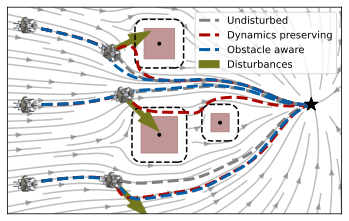
\includegraphics[width=0.95\columnwidth]{figures/multi_obstacle_with_damping.pdf}}
  % \centerline{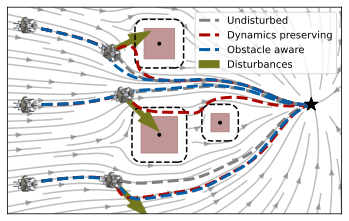
\includegraphics[width=0.5\textwidth]{figures/multi_obstacle_with_damping.svg}}
  \caption{The desired dynamics $\dot{\vecs \xi}$ in gray are as input for the force controller. 
  The mobile robot starting from the three positions, navigates safely to the attractor (black star) despite the disturbances (red arrows) when using the obstacle-aware controller.
  Conversely, the baseline (blue) leads to collision when the disturbance happens close to the robot.}
  \label{fig:obstacle_aware_damping_comparison}
\end{figure}

\subsection{Noise Analysis}
A real controller is always subject to noise, unexpected disturbances. This can be noise or inaccuracies in sensor readings, or small physical disturbances such as air drag for a fast moving drone, or floor roughness for a mobile robot. 
A high quality controller is able to reject such disturbances, while maintainingthe control ojbectives: collision avoidance and trajecotry tracking. 

This section looks at noise disturbance of a simulated agent with an identity mass matrix $\matd M = \matr I$. The discrete time step is chosen as $\Delta t = $\qty{0.2}{s}, furthermore the stiffness values are set as
$s^{\mathrm{obs}}=$\qty{50}{s^{-1}},
$s^{\mathrm{DS}}=$\qty{40}{s^{-1]}}, and
$s^{\mathrm{c}}=$\qty{5}{s^{-1}}.
% lambda_DS: 40.00
% lambda_perp: 5.00
% lambda_obs: 50.00
 The robot is tasked to follow a linear dynamics of  the form $\vect f(\vecs \xi) = (\vecs \xi^a -  \vecs \xi)$,nd the velocity is capped at a magnitude of \qty{1}{m/s}. 
 The controlless are compared by anaylyzing the minimal distance to the surface along a trajectory $ \min_t \| \vecs \xi_t - \vecs \xi^b \| $, see \eqref{eq:distance_function}.


\subsubsection{Velocity Noise Resistance}
In the first evaluation, normally distributed noise with mean of zero is added to the velocity $\dot{\vecs{ \xi}}$ before calulating the control force (Fig.~\ref{fig:velocity_noise}). Different variances of the noise are evaluated ranging from \qty{0}{m/s} to \qty{1.0}{m/s}. The start position is at $\vecs \xi_0 = [-2.5, 1.0]^T$ with an initial velocity of zero, and  the attractor at $\vecs \xi^a = [2.5, -1.0]^T$.
% The experiment is done on a simple setup with one obstacle. The noise added has a mean of $0$, and the standard deviation is increasing linearly from $0.0$ to $0.7m$ for position and $0.0$ to $7.0 \frac{m}{s}$ for velocity measurements. For each noise level, the simulation was run 10 times. The output variable is the smallest distance of the agent from the obstacle during the simulation. This metric was chosen to observe how the noise could lead to a crash in the obstacle. 

The obstacle aware controller is able to reject the noise acting on the velocity even with increasing noise variance. Nevertheless, the closest distance during the trajectory is decreasing with higerh values.
Conversely, the dynamics following has a mean distance which is below zero already at velocity noise variance of $\qty{0.5}{m/s}$, indicating a large number of trajectories colliding with at least one obstacle. 
It can futher be observed, without noise, the minimal distance along a trjaectory is higher for the obstacle aware controller. This is the result, that there is higher stiffness towards the obstacle, and hence the curvature of the dynamics guiding around the obstacle is followed more accurately.

\begin{figure}
    \centering
    \begin{subfigure}{\columnwidth}
      \centerline{\includegraphics[width=\textwidth]{figures/trajectory_velocity_noise}}
      \caption{Trajectories with a standard deviation of the velocity-noise of 1.0 m/s.}
      \label{fig:trajectory_velocity_noise}
    \end{subfigure}
    \begin{subfigure}{\columnwidth}
    \includegraphics[width=\textwidth]{figures/comparison_velocity_noise}
      \caption{The mean and variance (shaded) of the closest distances over 10 epochs.}
      \label{fig:comparison_velocity_noise}
    \end{subfigure}
	\caption{An agent is navigating towards the attractor (black star) between two elongated obstacles (a), while white noise acting on the agent's velocity. The velocity noise has a mean of zero, and different variances between \qty{0.0}{m / s} and \qty{1.0}{m / s} are evaluated.}
\label{fig:velocity_noise}
\end{figure}

\subsubsection{Position Noise Resistance} \label{sec:position_noise}
In the second experiment, normally distributed noise with mean of zero is added to the position $\vecs{ \xi}$ (Fig.~\ref{fig:position_noise}). The variances of the noise are ranging from \qty{0.0}{m/s} to \qty{0.3}{m/s}. The start position is at $\vecs \xi_0 = [-2.5, -1.0]^T$ with an initial velocity of zero, and  the attractor at $\vecs \xi^a = [2.5, 1.0]^T$.
% For the noise acting on the position measurement, the controller presents good rejection for a small noise variance. As it increases, the robot's behavior quickly worsens (Fig.~\ref{fig_pos_noise}). The robot penetrates the obstacle for noises of standard deviation $ > 0.4 m$. An example of a run with $\sigma_{noise} = 0.7 m$ is shown in Fig.~\ref{fig_pos_noise_0_7}.

% The obstacle was never penetrated for the velocity measurement noise, asserting the robustness of the control for this type of noise (Fig.~\ref{fig_vel_noise}). Fig.~\ref{fig_2_vel_noise} provides an image of the simulation with big noise standard deviation ($4.0 \frac{m}{s}$). Thanks to the feature presented in Section~\ref{sec:damping_only_toward} (damping only toward the obstacle), the robot has even the tendency to drift away from the obstacle, increasing the safety margin.
Similarly to the previous evaluatoin, the obstacle aware controller maintains a greater distance to the surface with zero noise, where the dynamics preserving already collides.
This results in the means of the  distance above zero for standard deviations of the position noise smaller than \qty{0.023}{m} using the obstacle aware controller. Whereas, for the dynamics preserving controller, the mean of the distance to the surface is below zero, indicating collisions.
However, this is the result of the buffer that comes from the obstacle aware controller. 
As a similar decrease in distance is detected for both controllers. 

Furthermore, a higher variance of the distance is observed in the dynamics preserving controller. We assume that this comes from the fact, that the higher impedance of this controller makes it slower to adapt to a new velocity after being displaced by the noise. Hence, the velocity and the trajectory is more random. 

\begin{figure}
    \centering
    \begin{subfigure}{\columnwidth}
      \centerline{\includegraphics[width=\textwidth]{figures/trajectory_position_noise}}
      \caption{Trajectories with a standard deviation of the position-noise of 0.0 m.}
      \label{fig:trajectory_position_noise}
    \end{subfigure}
    \begin{subfigure}{\columnwidth}
    \includegraphics[width=\textwidth]{figures/comparison_position_noise}
      \caption{Closest distances concerning different noise levels over 10 epochs.}
      \label{fig:comparison_position_noise}
    \end{subfigure}
	\caption{The agent is navigating towards the attractor (black star) between two concave obstacles (a), while white noise acting on the agent's position. The velocity noise has a mean of zero, different variances between \qty{0.0}{m} and \qty{0.03}{m} are evaluated.}
\label{fig:position_noise}
\end{figure}


\subsubsection{Obstacle Aware Passivity Using a Robot Arm}
The controller was used to guide a 7 degree of freedom robot arm (Pand from Franka Emika) while avoiding collisions. The state $\vect \xi$ of the robot is the end effectors positions, and the obtained control acceleration.final 

The joint torque is obtained using inverse kinemtatics:
\begin{equation}
	\vecs \tau_q = \matr J^{\dag}(\vect q) 
	\begin{bmatrix} \matd D(\vecs \xi) \left( \vect f(\vecs \xi) - \dot{\vecs \xi} \right) \\  p^\alpha (\vecs \alpha - \vecs \alpha^a) \end{bmatrix}
	% \;\; \text{with} \;\;
	% \matr J^{\dag} = \matr J^T (\matr J \matr J^T)^{-1}
\end{equation}
using the Moore-Penrose pseudo inverse of the Jacobian $\matr J^{\dag} = \matr J^T (\matr J \matr J^T)^{-1}$. The angle $\vecs \alpha$ describes the end effector orientation, and the desired orientation is pointing downward with a quaternio value of $\vecs \alpha^a = [0, 1, 0, 0]$. For the substraction, we use quaternion representation to avoid singularities, but for the evaluation of the torque from the angular offset angle-axis represtation of the orientation is used.

The angular stiffness is chosesn as $p^\alpha = 5.5$.
The damping values are set as
$s^{\mathrm{obs}}=\, $ \qty{160}{s^{-1}},
$s^{\mathrm{DS}}= \,$ \qty{64}{s^{-1]}}, and
$s^{\mathrm{c}}= \,$ \qty{16}{s^{-1}}.
% multiplier = 8.0  # increase for faster but less stable
% self.linear_principle_damping = 8 * multiplier  # 50.
% self.linear_obstacle_damping = 20 * multiplier  # 60.
% self.linear_orthogonal_damping = 2 * multiplier  # 20.


The robot was set to move from initial position approximately at $\vecs \xi_0 = [0.3\mathrm{m}, 0.4\mathrm{m}, 0.3\mathrm{m},]^T$ to the attractor $\vecs \xi^a = [0.26 \mathrm{m}, -0.53\mathrm{m}, 0.33\mathrm{m}]^T$.
The motion is guided by dynamical system in the presence of a single squared box with axes length \qty{0.16}{m}, and a margin of \qty{0.12}{m}. The box is placed approximately at the center of start and attractior, but the precise loaction  is obtained at each time step using marke based vision system (optitrack). 
While passing the box, the robot is disturbed by a strong push $\vecs t_e$ towards the box. The sequence is repeated 10 times for both controllers, as well as for the undisturbed motion.

From the experimental results in Figure~\ref{fig:evaluation_on_robot_arm}, it is observed that using the obstacle ware controller, the robot is able stay on average \qty{0.15}{m} away from the obstacle surface. While for the dynamics preserving controller, the mean distance is below \qty{0.05}{m}, and many trajectories collide with the box. 
This results from a much weaker control force of the obstacle aware controller. Which has a high peak as soon as the disturbance occurs, at around \qty{1.45}{s}. Conversely, for the dynamics preserving trajecotry no such high peak occurs, and the controller only acts when the robot is almost in collision. In fact, the obstacle aware controller already show high forces before the disturbance, this additionally results in improved tracking of the avoidance trajectory as we've seen in Section~\ref{sec:position_noise}.


\begin{figure}
    \centering
   \begin{subfigure}{\columnwidth}
    \includegraphics[width=0.49\textwidth]{figures/franka_sequence/franka_obstacle_aware016}\hfill%
    % \includegraphics[width=0.33\textwidth]{figures/franka_sequence/franka_obstacle_aware018}\hfill%
    \includegraphics[width=0.49\textwidth]{figures/franka_sequence/franka_obstacle_aware020}
      \caption{Obstacle aware controller rejects repulsion and avoids collision}
      \label{fig:franka_sequence_obstacle_aware}
    \end{subfigure}
	\begin{subfigure}{\columnwidth}
    \includegraphics[width=0.49\textwidth]{figures/franka_sequence/franka_velocity_conserving021}\hfill%
    % \includegraphics[width=-1.33\textwidth]{figures/franka_sequence/franka_velocity_conserving023}\hfill%
    \includegraphics[width=0.49\textwidth]{figures/franka_sequence/franka_velocity_conserving025}\hfill%
      \caption{Dynamics preserving controller leads to collsion with obstacle}
      \label{fig:franka_sequence_obstacle_aware}
    \end{subfigure}
%    \caption{Comparison of the two control methods}
%    \label{fig:evaluation_on_robot_arm}
% \end{figure}
% \begin{figure}
%     \centering
    \begin{subfigure}{\columnwidth}
      \centerline{\includegraphics[width=\textwidth]{figures/robot_arm_trajectory_xyz}}
      \caption{The two control methods compared with the undisturbed trajectory. Wider line indicates higher x-value. The darker arrow is the actual, and the brighter the desired velocity.}
      \label{fig:robot_arm_trajectory_xyz}
    \end{subfigure}
    \begin{subfigure}{\columnwidth}
		\includegraphics[width=\textwidth]{figures/trajectory_comparison_force_and_distance}
      \caption{The specific trajectory (full line), as well as average (dashed line) and variance (shaded area) over 10 runs are visualized. For the control force, mean and variance are evaluated in the logarithmic space.}
      \label{fig:trajectory_comparison_force_and_distance}
    \end{subfigure}
	\caption{Using the obstacle-aware passive controller, combined with a margin of 0.16m around the obstacle, the roboto arm is succesfully able to avoid the disturbance towards the obstacle. A similar disturbance has been applied to the robot arm over the 10 experimental runs. }  
    \label{fig:evaluation_on_robot_arm}
\end{figure}

\section{Discussion}
Overall, the simulated robot shows pleasing results. It has good tracking performances, compliance in the direction perpendicular to the motion, and great damping of the disturbances towards obstacles.
Away from obstacles, the controller presented shows similar behavior as the one in \cite{kronander2015passive}. When approaching one obstacle, the control gets stiffer to avoid collisions without losing its tracking properties. This makes the proposed controller a suitable option to cumulate good tracking and safety regarding obstacle penetration.

\subsection{Applicability Approach}
Note, that the theoretical analysis from Theorem~\ref{theorem:passivity}, indicates passivity for any velocity-bounded, uniquely damped system. As a result, work such as the damping-based controller in  \cite{kronander2015passive} does not require an energy tank anymore.
Conversely, if the impedance controller has a proportional $\mathcal{K}$, the adaptive proportional term might induce instabilities even for stable desired dynamics as pointed out in \cite{ferraguti2013tank, kronander2016stability}.


\appendix
%\section{Discrete Time Behavior} \label{sec:discrete_time_behavior}
So far, we've considered that the system is continuous time. 
This is a reasonable assumption, if we have a high sampling time $\Delta t$, compared to the dynamics, i.e., $\| \Delta t \, \dot{\vecs \xi} \| \ll 1$.
However, any digital controller sends a discrete control signal. In order to reject the disturbances in the presence of obstacles, a high control force is exerted (while still remaining within the control robot's limits), hence $\| \Delta t \, \vecs \tau^c \| \gg 1$. 
In this case, it is crucial to analyze the discrete-time system to guarantee stability, as high damping can lead to unstable behavior, see Figure~
\ref{fig:discrete_controller_parameters_comparison}).

\begin{figure}[htb]
\centering
  \includegraphics[width=\columnwidth]{figures/discrete_controller_parameters_comparison}
  \caption{A point-like agent with an initial velocity of $\{ \dot{\vecs \xi} \}_0 = [1 \; -1]^T$ is guided by the desired velocity $\vect f(\vecs \xi) = [1, 0]^T$, and a control matrix $\matd{D}$ with damping values $s_i$ equal in all directions, where $m$ is the mass of the point-like agent. 
  Damping values above $s_i = 2.0 m / \Delta t$ lead to unstable behavior where the higher value leads to higher oscillations. Conversely, the lowest value leads to more deviation from the straight trajectory resulting from the higher impedance. The critical value of $s_i = 2.0 m / \Delta t$ results in stable behavior with immediate correction to the desired velocity.}
  \label{fig:discrete_controller_parameters_comparison}
\end{figure}

For the discrete-time system, the position and velocity of the agent evolve as follows:
\begin{equation}
	\begin{bmatrix}
	 \vecs \xi_{t+1} \\ \dot{\vecs \xi}_{t+1}
	\end{bmatrix}
	=
	\begin{bmatrix}
	 \vecs \xi_{t} \\ \dot{\vecs \xi}_{t}
	\end{bmatrix}
	+ 
	\Delta t 
	\begin{bmatrix}
		\dot{\vecs \xi}_{t} \\ \ddot{\vecs \xi}_t 
	\end{bmatrix}
	\label{eq:discrete_time_dynamics}
\end{equation}

\begin{lemma}
	Let us consider a discrete-time system with state defined in Eq.~\eqref{eq:discrete_time_dynamics}, and is governed by the controller from Eq.~\eqref{eq:control_command} and damping matrix $\matd{D}$ defined in Eq.~\eqref{eq:damping_summation}.
	Let us consider the input the desired velocity $\vect f(\vecs \xi)$ and as output the agent's velocity $\dot{\vecs \xi}$. 
	The system is BIBO (bounded-input, bounded-stable) with respect to the velocity, i.e., $\lim_{t \rightarrow \infty} \| \dot{\vect \xi} \| < \infty$, if all eigenvalues of $\matd{M}^{-1} \matd{D}$ are less or equal to $2 / \Delta t$.
\end{lemma}

\begin{proof}
Hence, for the evaluation in discrete time, the evolution of the velocity is given by:
\begin{equation}
	\begin{split}
	& \begin{bmatrix}
	 \vecs \xi_{t+1} \\ \dot{\vecs \xi}_{t+1}
	\end{bmatrix}
	=
	\begin{bmatrix}
		\vect \xi_t + \Delta t  \; \dot{\vect \xi}_t \\ \
		\dot{\vecs \xi}_t + \Delta t \, \matd{M}^{-1} \left( \matd{D} \left( \vect f(\vecs \xi_t) - \dot{\vecs \xi}_t \right) - \matr C \right)
	\end{bmatrix} \\
	&  = %\approx
	\begin{bmatrix}
		\mathcal{I} & \mathcal{I} \Delta t \\
		\vect{0} & \mathcal{I} - \Delta t \matd{M}^{-1} \matd D 
	\end{bmatrix}
	\begin{bmatrix}
		\vect \xi_t \\ \dot{\vect \xi}_t
	\end{bmatrix}
	+ \begin{bmatrix}
		\vect{0} \\ 
		\Delta t \, \matd{M}^{-1} \matd{D} 
	\end{bmatrix}
	\hat{\vect f}(\vecs \xi_t) 
	% & \approx 
	% \begin{bmatrix}
	% 	1 & \Delta t \\
	% 	\Delta t \matd{M}^{-1} \matd D \frac{\partial \vect f}{\partial \vecs \xi} & 1 - \Delta t \matd{M}^{-1} \matd D 
	% \end{bmatrix}
	% \begin{bmatrix}
	% 	\vect \xi_t \\ \dot{\vect \xi}_t
	% \end{bmatrix}
	\label{eq:discrete_time_proof}
	\end{split}
\end{equation}
where $\hat{\vect f}(\vecs \xi_t) = \vect f(\vecs \xi_t) - \matd{D}^{-1} C$.  The state dependency of the matrices $\matd{M}$, $\matd{D}$, and $\matd{C}$ is omitted for brevity, and $\matd{I} \in \mathbb{R}^{N \times N}$ denotes the identity matrix.
As we look at global stability, the Coriolis acceleration $\matd{C}$ is merged into the dynamical system. Since the Coriolis force is bounded, it follows that if the system is BIBO stable for $\hat{\vect f}(\vect \xi)$ then it is also BIBO stable for $\vect f(\vecs \xi)$ 

% Let us introduce the coordinate transform $\dot{\vect \gamma}_t = \dot{\vect \xi}_t - \vect f(\vecs \xi)$  and hence for the position we have $\vect \gamma_t = \vect \xi_t - \Delta t \vect f(\vecs \xi)$, and hence 
% \begin{equation}
% 	\begin{split}
% 		\begin{bmatrix}
% 			\vect \gamma_{t+1} \\ \dot{\vect \gamma}_{t+1}
% 						\end{bmatrix}
% 	& =	
% 	\begin{bmatrix}
% 		1 & \Delta t \\
% 		0 & 1 - \Delta t \, \matd{M}^{-1} \matd{D}
% 	\end{bmatrix}
% 	\begin{bmatrix}
% 		\vecs \gamma_t \\ \dot{\vecs \gamma}_t
% 	\end{bmatrix}
% 	+ \begin{bmatrix} 
% 	\Delta t \vect f(\vecs \xi_t) \\ 0
%     \end{bmatrix} \\
% 	& \approx \begin{bmatrix}
% 		1 + \Delta t \frac{\partial \vect f}{\partial \vect \xi} & \Delta t \\
% 		0 & 1 - \Delta t \, \matd{M}^{-1} \matd{D}
% 	\end{bmatrix}
% 	\end{split}
% \end{equation}
% The summand $\vect t \vect f(\vecs \xi_t)$ changes the relative position value $\vect \gamma_t$ as long as the desired velocity is not zero. However, this only moves the relative position but does not influence kinetic energy, which has been used as the stability function (Section~\ref{sec:passivity_analysis}).

BIBO stability of a discrete-time system requires that all the eigenvalues of the feedback matrix are smaller or equal to one \cite{friedland2012control}.
The eigenvalues of the above feedback system are given as:
\begin{equation}
	\vect \lambda_1 = \text{eig}(\mathcal{I}) \qquad \vect \lambda_2 = \text{eig} \left(\mathcal{I} - \Delta t \, \matd{M}^{-1} \matd{D} \right)
\end{equation}
where both $\vect \lambda_1 \in \mathbb{R}^N$ and $\vect \lambda_2 \in \mathbb{R}^N$ denote a vector containing $N$ eigenvalues.
All eigenvalues of $\vect \lambda_{1, i} = 1, \; i = 1...N$, and hence are stable by the design of the system. 
The second set eigenvalues $\vect \lambda_2$  are dependent on the passive control term. 
However, since $\matd{M}$ and $\matd{D}$ are both positive definite, the eigenvalues are positive:
\begin{equation}
	\matd{M} > 0 \; , \;\; \matd{D} > 0 
	\qquad \Rightarrow \qquad
	\lambda_{2, i} > 0 \quad i = 1...N
\end{equation}
% Furthermore, the system is stable if all eigenvalues are smaller or equal to one \cite{friedland2012control}. 
Hence, the system is stable if the maximum eigenvalue is limited as:
\begin{equation}
	\max \left(\vect \lambda_2 \right) \leq 1 
	\quad \Rightarrow \quad
	\max \Bigl( \text{eig}\bigl(\matd{M}^{-1} \matd{D} \bigr)  \Bigr) \leq 2 / \Delta t
\end{equation}
\end{proof}


\subsection{Asymptotic Stability}
The stability guarantees in the previous section; the system's stability was reduced to boundedness. 
Since the first eigenvalue equals one, asymptotic convergence does not occur. 
This implies that if the input goes to zero, i.e., $\vect f(\vecs \xi) = \vect 0$, the system stops and does not converge to a specified point. Since the desired velocity should only reach zero at the attractor, the system is expected to converge in most cases.

Yet, asymptotic stability is not guaranteed for general nonlinear input dynamics. Especially for dynamics with high curvature and low damping value, the final trajectory can end up in limit cycles ((Figure~\ref{fig:discrete_controller_parameters_comparison_stable}).

\begin{figure}[htb]
\centering
  \includegraphics[width=\columnwidth]{figures/discrete_controller_parameters_comparison_stable}
\caption{A point-like agent which is following the desired dynamics of
$\vect f(\vecs \xi) = \matr R(\pi / 6) (\vect \xi  - \vect \xi^a)$ where $\matr R(\cdot)$ is the rotation matrix, and with equal damping values $s_i$, where $m$ is the mass of the agent.
The controller with a critical stiffness of $2.0 m / \Delta t$ leads to fast convergence and a stable system. With lower damping (top left), there is a large drift of the system and the system converges to a limit cycle. 
The high damping of $2.3 m / \Delta t$ leads to an unstable system. 
Interestingly, with stiffness of $2.1 m / \Delta t$ in combination, we obtain a visibly stable system.}
  \label{fig:discrete_controller_parameters_comparison_stable}
\end{figure}

% For a general nonlinear system no asymptotic convergence evaluation can be made. This is due to the fact, that for any system there is a slight drift due to the damping values.
% And hence, if there are high nonlinearities in the system it could happen that even with a stable system, the dynamics get caught in a limit cycle. However, for most common globally asymptotic systems (for velocity-position), the force controller as proposed leads to globally asymptotically stable behavior, too (Figure~\ref{fig:discrete_controller_parameters_comparison_stable}).

% \subsection{Intertial Drift}
% Let us assume that have strong damping in the direction of the obstacle, i.e., $s^{\mathrm{obs}} / m_i \gg 1$, where $m_i$ with $i = 1, .., N$ represent the eigenvalues of the mass matrix $\matd{M}$. 
% 

\section{Discrete Time Behavior} \label{sec:discrete_time_behavior}
So far, we've considered that the system is continuous time. 
This is a reasonable assumption, if we have a high sampling time $\Delta t$, compared to the dynamics, i.e., $\| \Delta t \, \dot{\vecs \xi} \| \ll 1$.
However, any digital controller sends a discrete control signal. In order to reject the disturbances in the presence of obstacles, a high control force is exerted (while still remaining within the control robot's limits), hence $\| \Delta t \, \vecs \tau^c \| \gg 1$. 
In this case, it is crucial to analyze the discrete-time system to guarantee stability, as high damping can lead to unstable behavior, see Figure~
\ref{fig:discrete_controller_parameters_comparison}).

\begin{figure}[htb]
\centering
  \includegraphics[width=\columnwidth]{figures/discrete_controller_parameters_comparison}
  \caption{A point-like agent with an initial velocity of $\{ \dot{\vecs \xi} \}_0 = [1 \; -1]^T$ is guided by the desired velocity $\vect f(\vecs \xi) = [1, 0]^T$, and a control matrix $\matd{D}$ with damping values $s_i$ equal in all directions, where $m$ is the mass of the point-like agent. 
  Damping values above $s_i = 2.0 m / \Delta t$ lead to unstable behavior where the higher value leads to higher oscillations. Conversely, the lowest value leads to more deviation from the straight trajectory resulting from the higher impedance. The critical value of $s_i = 2.0 m / \Delta t$ results in stable behavior with immediate correction to the desired velocity.}
  \label{fig:discrete_controller_parameters_comparison}
\end{figure}

For the discrete-time system, the position and velocity of the agent evolve as follows:
\begin{equation}
	\begin{bmatrix}
	 \vecs \xi_{t+1} \\ \dot{\vecs \xi}_{t+1}
	\end{bmatrix}
	=
	\begin{bmatrix}
	 \vecs \xi_{t} \\ \dot{\vecs \xi}_{t}
	\end{bmatrix}
	+ 
	\Delta t 
	\begin{bmatrix}
		\dot{\vecs \xi}_{t} \\ \ddot{\vecs \xi}_t 
	\end{bmatrix}
	\label{eq:discrete_time_dynamics}
\end{equation}

\begin{lemma}
	Let us consider a discrete-time system with state defined in Eq.~\eqref{eq:discrete_time_dynamics}, and is governed by the controller from Eq.~\eqref{eq:control_command} and damping matrix $\matd{D}$ defined in Eq.~\eqref{eq:damping_summation}.
	Let us consider the input the desired velocity $\vect f(\vecs \xi)$ and as output the agent's velocity $\dot{\vecs \xi}$. 
	The system is BIBO (bounded-input, bounded-stable) with respect to the velocity, i.e., $\lim_{t \rightarrow \infty} \| \dot{\vect \xi} \| < \infty$, if all eigenvalues of $\matd{M}^{-1} \matd{D}$ are less or equal to $2 / \Delta t$.
\end{lemma}

\begin{proof}
Hence, for the evaluation in discrete time, the evolution of the velocity is given by:
\begin{equation}
	\begin{split}
	& \begin{bmatrix}
	 \vecs \xi_{t+1} \\ \dot{\vecs \xi}_{t+1}
	\end{bmatrix}
	=
	\begin{bmatrix}
		\vect \xi_t + \Delta t  \; \dot{\vect \xi}_t \\ \
		\dot{\vecs \xi}_t + \Delta t \, \matd{M}^{-1} \left( \matd{D} \left( \vect f(\vecs \xi_t) - \dot{\vecs \xi}_t \right) - \matr C \right)
	\end{bmatrix} \\
	&  = %\approx
	\begin{bmatrix}
		\mathcal{I} & \mathcal{I} \Delta t \\
		\vect{0} & \mathcal{I} - \Delta t \matd{M}^{-1} \matd D 
	\end{bmatrix}
	\begin{bmatrix}
		\vect \xi_t \\ \dot{\vect \xi}_t
	\end{bmatrix}
	+ \begin{bmatrix}
		\vect{0} \\ 
		\Delta t \, \matd{M}^{-1} \matd{D} 
	\end{bmatrix}
	\hat{\vect f}(\vecs \xi_t) 
	% & \approx 
	% \begin{bmatrix}
	% 	1 & \Delta t \\
	% 	\Delta t \matd{M}^{-1} \matd D \frac{\partial \vect f}{\partial \vecs \xi} & 1 - \Delta t \matd{M}^{-1} \matd D 
	% \end{bmatrix}
	% \begin{bmatrix}
	% 	\vect \xi_t \\ \dot{\vect \xi}_t
	% \end{bmatrix}
	\label{eq:discrete_time_proof}
	\end{split}
\end{equation}
where $\hat{\vect f}(\vecs \xi_t) = \vect f(\vecs \xi_t) - \matd{D}^{-1} C$.  The state dependency of the matrices $\matd{M}$, $\matd{D}$, and $\matd{C}$ is omitted for brevity, and $\matd{I} \in \mathbb{R}^{N \times N}$ denotes the identity matrix.
As we look at global stability, the Coriolis acceleration $\matd{C}$ is merged into the dynamical system. Since the Coriolis force is bounded, it follows that if the system is BIBO stable for $\hat{\vect f}(\vect \xi)$ then it is also BIBO stable for $\vect f(\vecs \xi)$ 

% Let us introduce the coordinate transform $\dot{\vect \gamma}_t = \dot{\vect \xi}_t - \vect f(\vecs \xi)$  and hence for the position we have $\vect \gamma_t = \vect \xi_t - \Delta t \vect f(\vecs \xi)$, and hence 
% \begin{equation}
% 	\begin{split}
% 		\begin{bmatrix}
% 			\vect \gamma_{t+1} \\ \dot{\vect \gamma}_{t+1}
% 						\end{bmatrix}
% 	& =	
% 	\begin{bmatrix}
% 		1 & \Delta t \\
% 		0 & 1 - \Delta t \, \matd{M}^{-1} \matd{D}
% 	\end{bmatrix}
% 	\begin{bmatrix}
% 		\vecs \gamma_t \\ \dot{\vecs \gamma}_t
% 	\end{bmatrix}
% 	+ \begin{bmatrix} 
% 	\Delta t \vect f(\vecs \xi_t) \\ 0
%     \end{bmatrix} \\
% 	& \approx \begin{bmatrix}
% 		1 + \Delta t \frac{\partial \vect f}{\partial \vect \xi} & \Delta t \\
% 		0 & 1 - \Delta t \, \matd{M}^{-1} \matd{D}
% 	\end{bmatrix}
% 	\end{split}
% \end{equation}
% The summand $\vect t \vect f(\vecs \xi_t)$ changes the relative position value $\vect \gamma_t$ as long as the desired velocity is not zero. However, this only moves the relative position but does not influence kinetic energy, which has been used as the stability function (Section~\ref{sec:passivity_analysis}).

BIBO stability of a discrete-time system requires that all the eigenvalues of the feedback matrix are smaller or equal to one \cite{friedland2012control}.
The eigenvalues of the above feedback system are given as:
\begin{equation}
	\vect \lambda_1 = \text{eig}(\mathcal{I}) \qquad \vect \lambda_2 = \text{eig} \left(\mathcal{I} - \Delta t \, \matd{M}^{-1} \matd{D} \right)
\end{equation}
where both $\vect \lambda_1 \in \mathbb{R}^N$ and $\vect \lambda_2 \in \mathbb{R}^N$ denote a vector containing $N$ eigenvalues.
All eigenvalues of $\vect \lambda_{1, i} = 1, \; i = 1...N$, and hence are stable by the design of the system. 
The second set eigenvalues $\vect \lambda_2$  are dependent on the passive control term. 
However, since $\matd{M}$ and $\matd{D}$ are both positive definite, the eigenvalues are positive:
\begin{equation}
	\matd{M} > 0 \; , \;\; \matd{D} > 0 
	\qquad \Rightarrow \qquad
	\lambda_{2, i} > 0 \quad i = 1...N
\end{equation}
% Furthermore, the system is stable if all eigenvalues are smaller or equal to one \cite{friedland2012control}. 
Hence, the system is stable if the maximum eigenvalue is limited as:
\begin{equation}
	\max \left(\vect \lambda_2 \right) \leq 1 
	\quad \Rightarrow \quad
	\max \Bigl( \text{eig}\bigl(\matd{M}^{-1} \matd{D} \bigr)  \Bigr) \leq 2 / \Delta t
\end{equation}
\end{proof}


\subsection{Asymptotic Stability}
The stability guarantees in the previous section; the system's stability was reduced to boundedness. 
Since the first eigenvalue equals one, asymptotic convergence does not occur. 
This implies that if the input goes to zero, i.e., $\vect f(\vecs \xi) = \vect 0$, the system stops and does not converge to a specified point. Since the desired velocity should only reach zero at the attractor, the system is expected to converge in most cases.

Yet, asymptotic stability is not guaranteed for general nonlinear input dynamics. Especially for dynamics with high curvature and low damping value, the final trajectory can end up in limit cycles ((Figure~\ref{fig:discrete_controller_parameters_comparison_stable}).

\begin{figure}[htb]
\centering
  \includegraphics[width=\columnwidth]{figures/discrete_controller_parameters_comparison_stable}
\caption{A point-like agent which is following the desired dynamics of
$\vect f(\vecs \xi) = \matr R(\pi / 6) (\vect \xi  - \vect \xi^a)$ where $\matr R(\cdot)$ is the rotation matrix, and with equal damping values $s_i$, where $m$ is the mass of the agent.
The controller with a critical stiffness of $2.0 m / \Delta t$ leads to fast convergence and a stable system. With lower damping (top left), there is a large drift of the system and the system converges to a limit cycle. 
The high damping of $2.3 m / \Delta t$ leads to an unstable system. 
Interestingly, with stiffness of $2.1 m / \Delta t$ in combination, we obtain a visibly stable system.}
  \label{fig:discrete_controller_parameters_comparison_stable}
\end{figure}

% For a general nonlinear system no asymptotic convergence evaluation can be made. This is due to the fact, that for any system there is a slight drift due to the damping values.
% And hence, if there are high nonlinearities in the system it could happen that even with a stable system, the dynamics get caught in a limit cycle. However, for most common globally asymptotic systems (for velocity-position), the force controller as proposed leads to globally asymptotically stable behavior, too (Figure~\ref{fig:discrete_controller_parameters_comparison_stable}).

% \subsection{Intertial Drift}
% Let us assume that have strong damping in the direction of the obstacle, i.e., $s^{\mathrm{obs}} / m_i \gg 1$, where $m_i$ with $i = 1, .., N$ represent the eigenvalues of the mass matrix $\matd{M}$. 
% 


\renewcommand*{\bibfont}{\footnotesize}
\printbibliography

\end{document}
